\documentclass[oneside,a4paper,14pt]{extarticle}
\usepackage[T1,T2A,TU]{fontenc}
\usepackage[a4paper,letterpaper,top=20mm,bottom=20mm,left=20mm,right=10mm]{geometry}
\usepackage[russian]{babel}
\usepackage{textcomp}
\usepackage{indentfirst}
\usepackage{graphicx}
\usepackage{mwe}
\usepackage{wrapfig}
\usepackage{caption}
\usepackage{amsmath}
\usepackage{amsfonts}
\usepackage{amsthm}
\usepackage{amssymb}
\usepackage[all]{xy}
\usepackage[breaklinks]{hyperref}
\usepackage{titlesec}
\usepackage{verbatim, fancyvrb}

\titleformat{\section} % Настройка формата заголовков секций
{\normalsize\bfseries} % Устанавливает размер шрифта на нормальный и делает его жирным
{\thesection} % Указывает, что номер секции будет отображаться перед заголовком
{1em} % Устанавливает расстояние между номером секции и заголовком в 1em
{} % Дополнительные параметры.

\titleformat{\subsection} % Настройка формата заголовков подсекций
{\normalsize\bfseries} % Устанавливает размер шрифта на нормальный и делает его жирным
{\thesubsection} % Указывает, что номер подсекции будет отображаться перед заголовком
{1em} % Устанавливает расстояние между номером подсекции и заголовком в 1em
{} % Дополнительные параметры.

\titleformat{\subsubsection} % Настройка формата заголовков подподсекций
{\normalsize\bfseries} % Устанавливает размер шрифта на нормальный и делает его жирным
{\thesubsection} % Указывает, что номер подподсекции будет отображаться перед заголовком
{1em} % Устанавливает расстояние между номером подподсекции и заголовком в 1em
{} % Дополнительные параметры.

\renewcommand\baselinestretch{1.45}\normalsize %межстр интервал
\setlength{\parindent}{1.25cm} %длина отступа нового абзаца

\begin{document}
\newpage
\thispagestyle{empty}
\begin{center}
	МИНИСТЕРСТВО НАУКИ И ВЫСШЕГО ОБРАЗОВАНИЯ\\
	РОССИЙСКОЙ ФЕДЕРАЦИИ
	ФЕДЕРАЛЬНОЕ ГОСУДАРСТВЕННОЕ БЮДЖЕТНОЕ\\
	ОБРАЗОВАТЕЛЬНОЕ
	УЧРЕЖДЕНИЕ ВЫСШЕГО ОБРАЗОВАНИЯ\\
	«ВЯТСКИЙ ГОСУДАРСТВЕННЫЙ УНИВЕРСИТЕТ»\\
	Институт математики и информационных систем\\
	Факультет автоматики и вычислительной техники\\
	Кафедра электронных вычислительных машин
\end{center}
\vspace{20mm}

\begin{center}
	Отчёт по лабораторной работе №2\\
	по дисциплине\\
	<<Программирование>>\\
\end{center}
\vspace{40mm}
\noindent
\begin{tabular}{ll}
	Разработал студент гр. ИВТб-1301-05-00 & \rule[-1mm]{30mm}{0.10mm}\,/Черкасов А. А./   \\
	                                       & \hspace{8mm}\footnotesize(подпись)            \\

	Заместитель кафедры ЭВМ                & \rule[-1mm]{30mm}{0.10mm}\,/Долженкова М. Л./ \\
	                                       & \hspace{8mm}\footnotesize(подпись)            \\
\end{tabular}

\vfill
\begin{center}
	Киров\\
	2024
\end{center}

\newpage\thispagestyle{plain}

\section*{Цель}

\sloppy Цель работы: изучение и применение основ программирования на языках Pascal и C через выполнение практических заданий, направленных на развитие навыков алгоритмического мышления, освоение синтаксиса языков, а также на решение задач, связанных с обработкой данных и реализацией алгоритмов.

\section*{Задания}

\begin{enumerate}
	\item \textbf{Сумма двух предыдущих.} \\
	      Задан числовой одномерный массив-кольцо, насчитывающий N элементов. Вместо каждого элемента с нулевым значением поставить сумму двух предыдущих элементов массива. Гарантируете, что количество элементов в массиве не менее трех.\\
	      \textbf{Формат ввода.} \\
	      В первой строке вводится натуральное число N - количество элементов в массиве. Во второй строке элементы массива через пробел.\\
	      \textbf{Формат вывода.} \\
	      В строке выводится новый массив элементов, разделяемых пробелом
	      $$
		      \begin{tabular}{ll}
			      \textbf{Ввод} & \textbf{Вывод} \\
			      \hline
			      3             & 3 1 2          \\
			      0 1 2         &                \\
			      \hline
		      \end{tabular}
	      $$

	\item \textbf{Убывающая последовательность.} \\
	      Дан одномерный массив из N элементов. Определить, образуют ли элементы массива расположенные перед первым отрицательным числом, убывающую последовательность.\\
	      \newpage
	      \textbf{Формат ввода.} \\
	      В первой строке вводится число N количество элементов в исходном массиве. Во второй строке через пробел задаются элементы массива.\\
	      \textbf{Формат вывода.}\\
	      Вывести Yes - если найдена убывающая поcледовавтельность и No - в любом другом случае.\\
	      $$
		      \begin{tabular}{ll}
			      \textbf{Ввод}             & \textbf{Вывод} \\
			      \hline
			      3                         & Yes            \\
			      19 10 -4                  &                \\
			      \hline
			      8                         & No             \\
			      15 6 23 -19 -25 -4 -25 29 &                \\
			      \hline
		      \end{tabular}
	      $$

	\item \textbf{Единицы.} \\
	      Дан массив из N чисел, содержащий только нули и единицы. Найти номер элемента с которого начинается самая длинная последовательность единиц и количество элементов этой последовательности. Если таких последовательностей несколько, вывести номер последней из них. Если единицы в исходном массиве отсутствуют - вывести дважды 0. \\
	      \textbf{Формат ввода.} \\
	      В первой строке вводится число N количество элементов в исходном массиве. Во второй строке через пробел задаются элементы массива.\\
	      \textbf{Формат вывода.}\\
	      В единственной строке через пробел записываются два целых числа - номер элемента (начиная с нулевого) с которого начинается последовательность единиц и длинна максимальной последовательности. Или 0 0 - если единиц в исходном массиве нет. \\
	      $$
		      \begin{tabular}{ll}
			      \textbf{Ввод}                   & \textbf{Вывод} \\
			      \hline
			      16                              & 11 2           \\
			      0 1 1 0 1 0 0 1 0 1 0 1 1 0 0 1 &                \\
			      \hline
		      \end{tabular}
	      $$
	\item \textbf{Меньше правого соседа.} \\
	      Дан массив из N целых чисел. Сформировать новый массив, состоящий из элементов исходного массив, значения которых меньше их правого соседа. \\
	      \textbf{Формат ввода.} \\
	      В первой строке задается число N - количество элементов исходного массива Во второй строке через пробел задаются элементы массива. \\
	      \textbf{Формат вывода.}\\
	      В первой строке выводится длина нового массива Во второй строке элементы нового массива через пробел Если элементов удовлетворяющих условию нет, то в первой строке выводится NO, а вторая строка отсутсвует. \\
	      $$
		      \begin{tabular}{ll}
			      \textbf{Ввод}                      & \textbf{Вывод}  \\
			      \hline
			      15                                 & 5               \\
			      9 -1 -3 -1 7 1 3 3 3 7 4 1 5 4 -10 & -3 -1 1 3 1     \\
			      \hline
			      11                                 & 6               \\
			      -8 8 -1 10 0 1 6 -8 -5 5 -6        & -8 -1 0 1 -8 -5 \\
			      \hline
		      \end{tabular}
	      $$
	\item \textbf{Меньше K.} \\
	      В массиве из N целых чисел выбрать максимальное количество подряд
	      идущих элементов, сумма которых не превышала бы целого числа K. \\
	      \textbf{Формат ввода.} \\
	      В первой строке вводится число N количество элементов в исходном
	      массиве и число K. Во второй строке через пробел задаются элементы
	      массива. \\
	      \textbf{Формат вывода.}\\
	      В единственной строке указать число соответствующее максимальному
	      количеству элементов, удовлетворяющих условию. \\
	      $$
		      \begin{tabular}{ll}
			      \textbf{Ввод}                                   & \textbf{Вывод} \\
			      \hline
			      2 18                                            & 2              \\
			      14 -24                                          &                \\
			      \hline
			      16 14                                           & 10             \\
			      7 8 -4 24 -25 -7 -8 12 22 -11 25 -18 15 25 5 15 &                \\
			      \hline
		      \end{tabular}
	      $$
	\item \textbf{Расширение массива.} \\
	      В заданном одномерном массиве, состоящем из N целых чисел
	      подсчитать количество элементов, делящихся нацело на 3, и целую часть
	      (округление по правилам арифметики) среднего арифметического элементов с
	      чётными значениями. Поставить полученные величины на первое и последнее
	      места в исходном массиве (увеличить массив на 2 элемента). \\
	      \textbf{Формат ввода.} \\
	      В первой строке задается натуральное число N $\leq $
	      200 - количество элементов в исходном массиве. Во второй строке элементы
	      массива, разделяемые пробелом.\\
	      \textbf{Формат вывода.}\\
	      В единственной строке вывести новый массив, элементы которого
	      разделены пробелом.\\
	      $$
		      \begin{tabular}{ll}
			      \textbf{Ввод} & \textbf{Вывод}  \\
			      \hline
			      4             & 1 5 17 -18 2 -8 \\
			      5 17 -18 2    &                 \\
			      \hline
		      \end{tabular}
	      $$
	\item \textbf{Матрица средних.} \\
	      В прямоугольной матрице A, имеющей N строк и M столбцов найти
	      наименьшее значение среди средних значений для каждой строки матрицы. \\
	      \textbf{Формат ввода.} \\
	      В первой строке вводятся числа N и M - количество строк и столбцов
	      матрицы В следующих последовательных N строках вводятся через пробел
	      элементы срок матрицы, начиная с первой строки.\\
	      \textbf{Формат вывода.}\\
	      Единственное число соответствующее среднему значению, округленному
	      до двух знаков после запятой. \\
	      $$
		      \begin{tabular}{ll}
			      \textbf{Ввод} & \textbf{Вывод} \\
			      \hline
			      3 4           & 0.50           \\
			      10 5 -4 2     &                \\
			      1 8 6 -13     &                \\
			      5 2 7 9       &                \\
			      \hline
		      \end{tabular}
	      $$
	\item \textbf{Между нулями.} \\
	      Дан массив из N целых чисел, содержащий по крайней мере два нуля.
	      Вывести сумму чисел из данного массива, расположенных между двумя
	      последними нулями.\\
	      \textbf{Формат ввода.} \\
	      В первой строке число N - количество элементов массива Во второй строке
	      целые элементы массива через пробел. \\
	      \textbf{Формат вывода.}\\
	      Вывести единственное целое число, соответствующее искомой сумме. \\
	      $$
		      \begin{tabular}{ll}
			      \textbf{Ввод}                    & \textbf{Вывод} \\
			      \hline
			      9                                & 0              \\
			      19 10 16 10 1 20 10 0 0          &                \\
			      \hline
			      13                               & 18             \\
			      1 11 13 0 18 20 0 18 21 0 18 0 1 &                \\
			      \hline
			      13                               & 141            \\
			      0 14 7 11 19 1 21 14 6 4 21 23 0 &                \\
			      \hline
		      \end{tabular}
	      $$
	\item \textbf{Рыба-пила.} \\
	      Дан массив из N вещественных чисел (N < 100). Будем называть
	      массив пилообразным, если каждый его внутренний элемент либо больше, либо
	      меньше обоих его соседей. Например, массив 1 5 2 4 3 7 5 - пилообразный.\\
	      \textbf{Формат ввода.} \\
	      В первой строке вводится число N - количество элементов в массиве
	      Во второй строке вводятся через пробел элементы массива.\\
	      \textbf{Формат вывода.}\\
	      Вывести Yes - если массив пилообразный и No в противном случае. \\
	      $$
		      \begin{tabular}{ll}
			      \textbf{Ввод} & \textbf{Вывод} \\
			      \hline
			      5             & Yes            \\
			      1 0 1 0 1     &                \\
			      \hline
		      \end{tabular}
	      $$
	\item \textbf{Нарушение закономерности.}\\
	      Дан массив из N вещественных чисел. Если данный массив образует
	      неубывающую последовательности , то вывести 0. В противном случае вывести
	      номер первого числа (нумерация начинается с нуля) нарушающего
	      закономерность. \\
	      \textbf{Формат ввода.} \\
	      В первой строке вводится число N - количество элементов в массиве. Во
	      второй строке через пробел вводятся вещественные числа образующие массив. \\
	      \textbf{Формат вывода.}\\
	      Вывести 0 или номер элемента нарушающего закономерность. \\
	      $$
		      \begin{tabular}{ll}
			      \textbf{Ввод}                            & \textbf{Вывод} \\
			      \hline
			      15                                       & 2              \\
			      -4.23 5.14 -1.94 6.39 -5.90 -7.38 -8.42  &                \\
			      -0.60 6.55 3.65 -5.96 8.27 1.8 -4.5 1.58 &                \\
			      \hline
		      \end{tabular}
	      $$
\end{enumerate}

\section*{Задание 1.}
\noindent Схема алгоритма Задания 1 представлена на Рисунке 1.\\
\noindent Исходный код представлен в Приложении А1. \\
\begin{figure}[!ht]
	\centering
	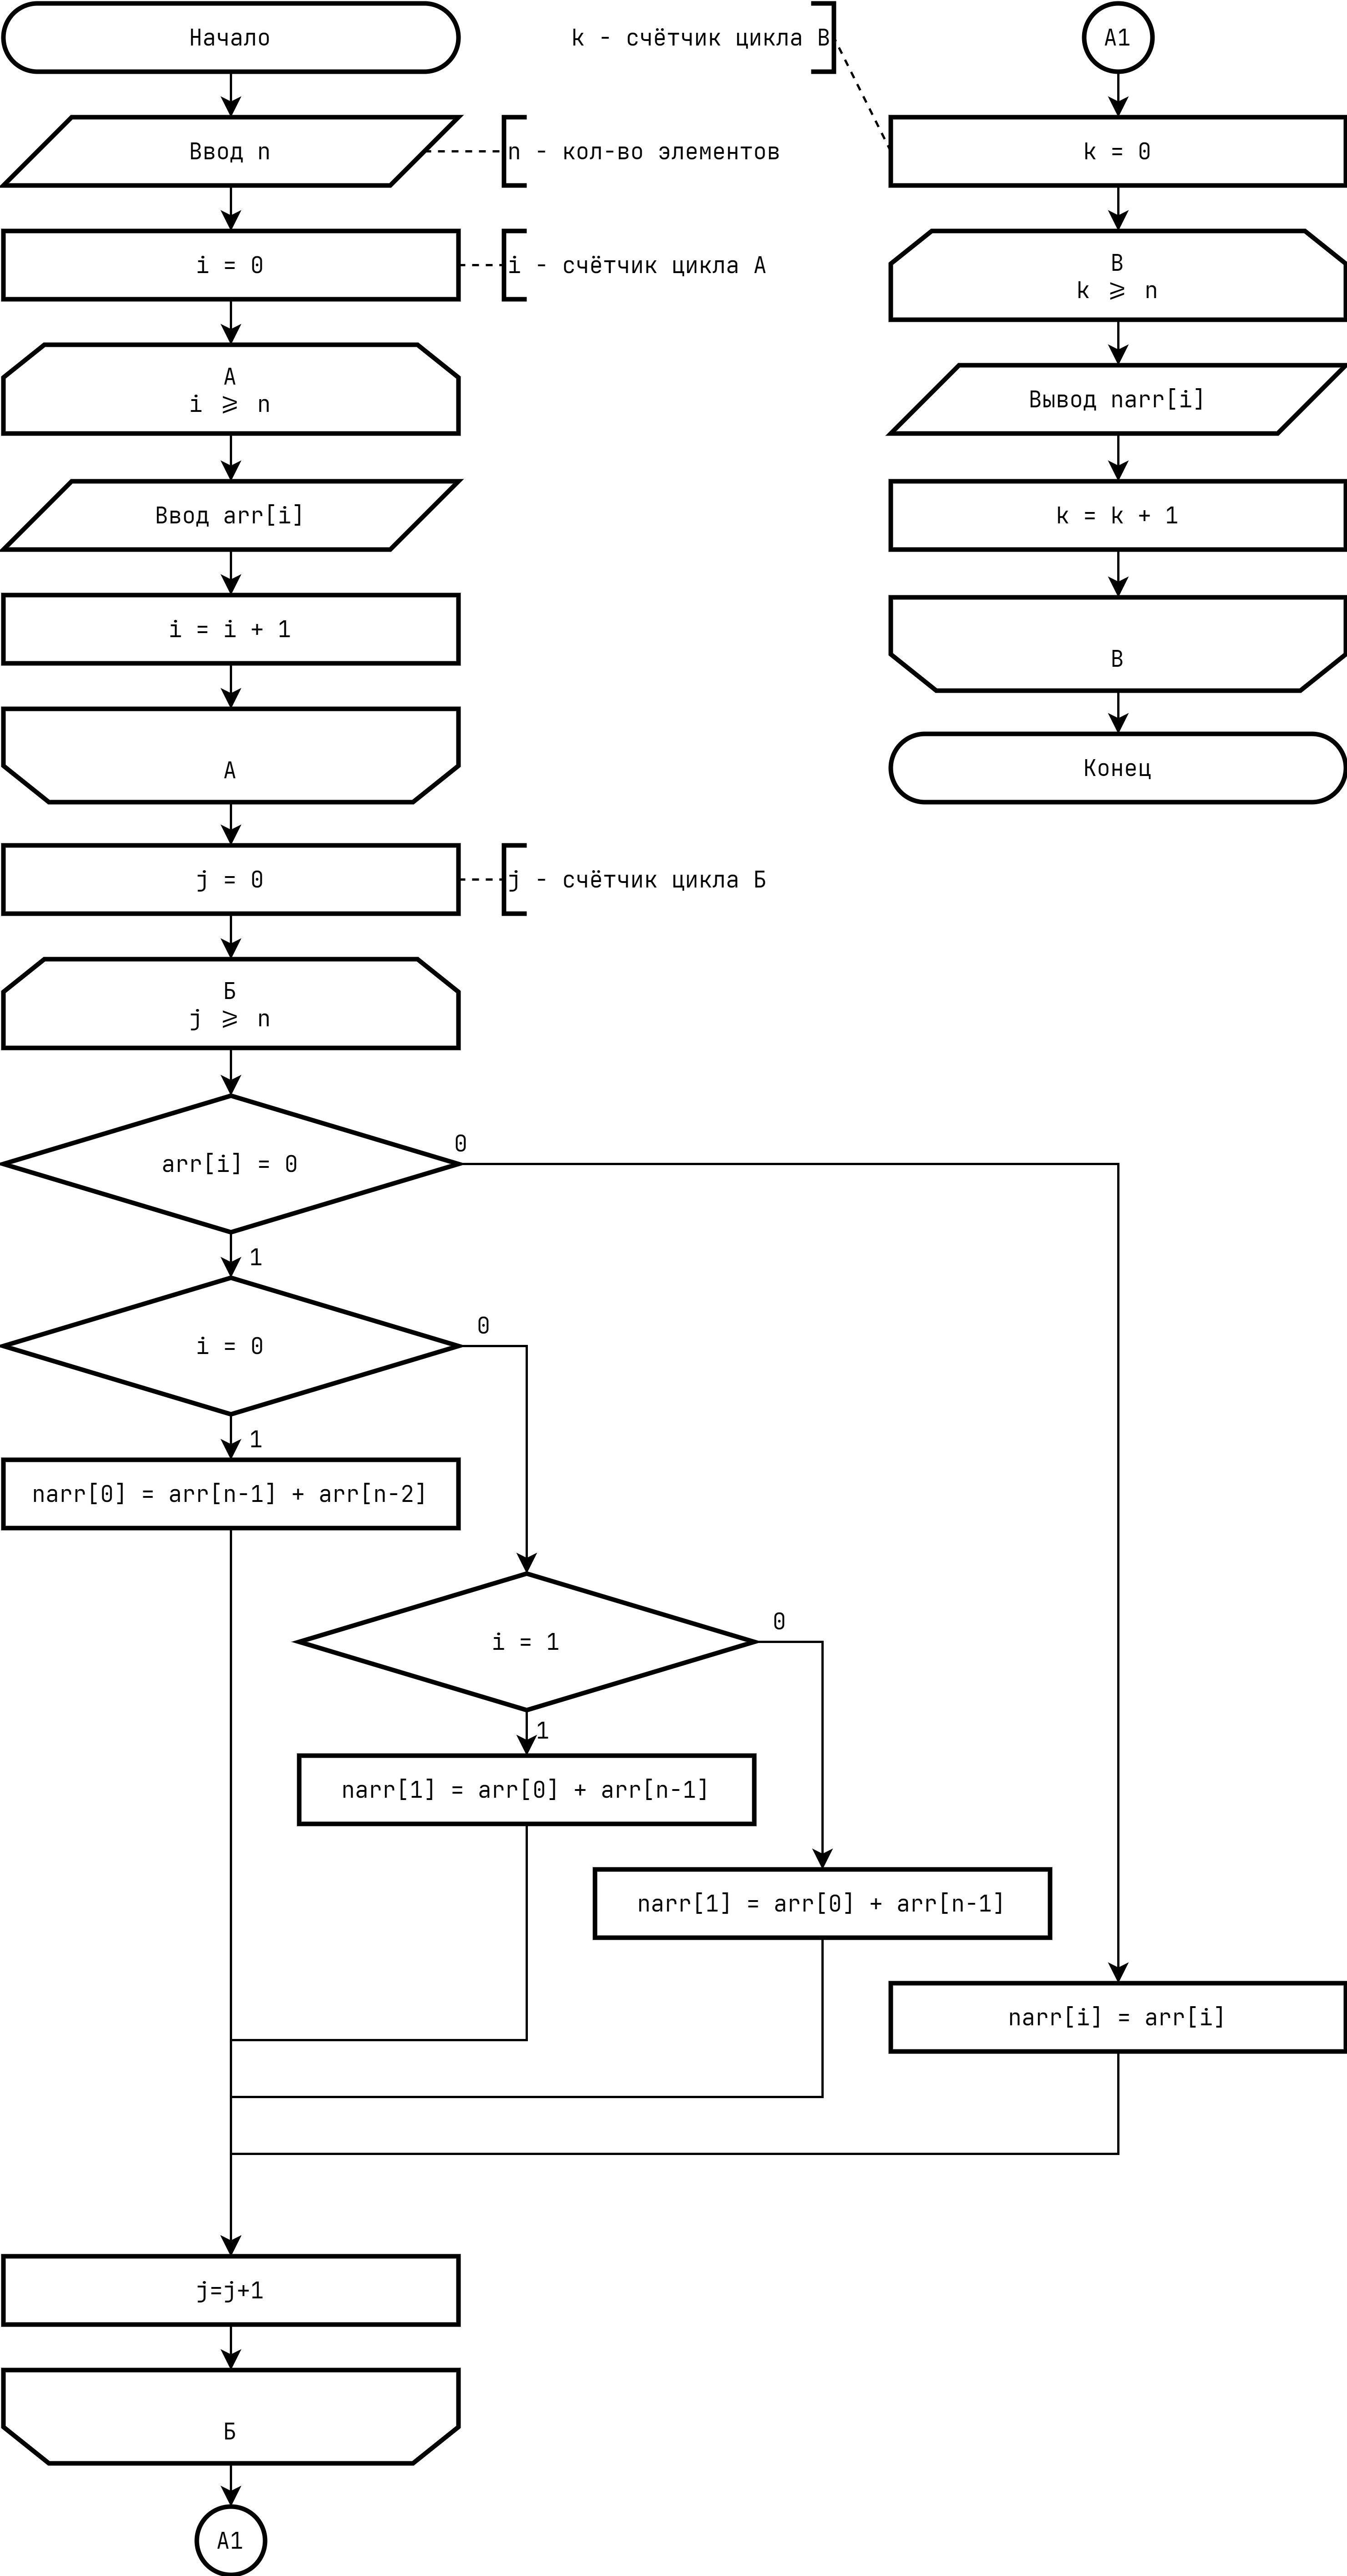
\includegraphics[width=0.5\textwidth]{pics/flowchart-13.png}
	\caption*{Рисунок 1 - Схема алгоритма Задания 1.}
\end{figure}

\section*{Задание 2.}
\noindent Схема алгоритма Задания 2 представлена на Рисунке 2.\\
\noindent Исходный код представлен в Приложении А2. \\

\begin{figure}[!ht]
	\centering
	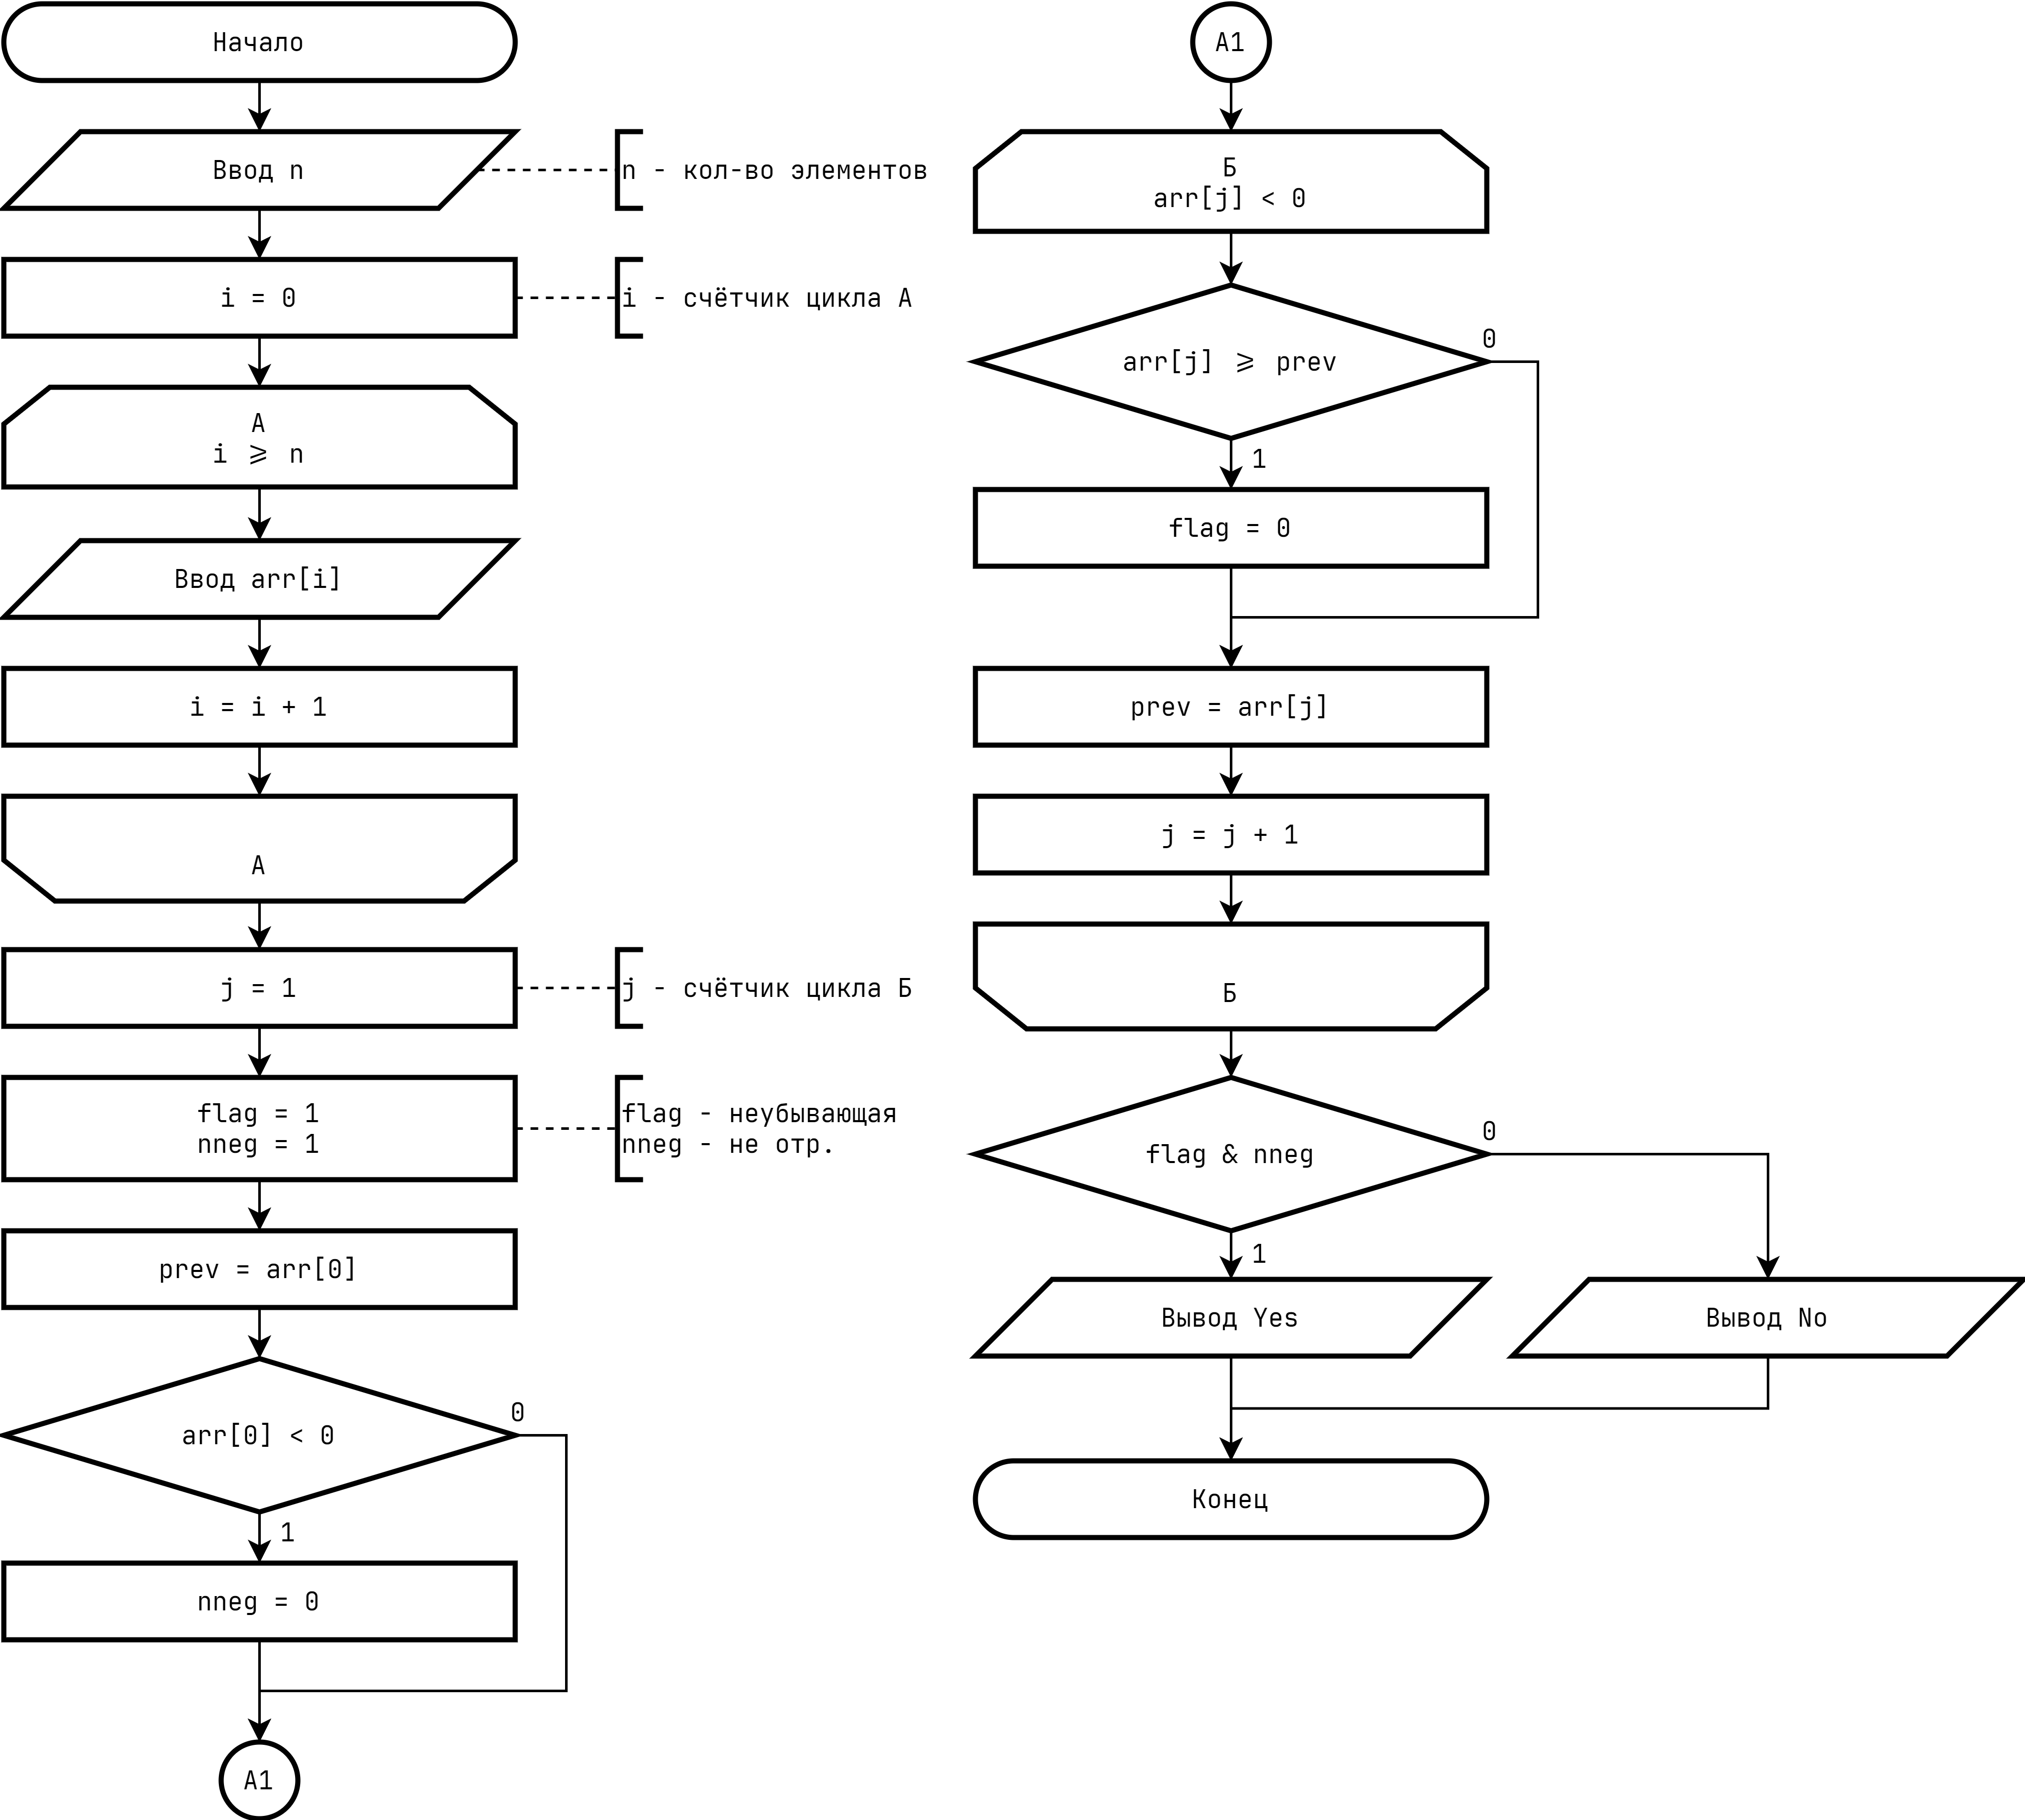
\includegraphics[width=0.75\textwidth]{pics/flowchart-14.png}
	\caption*{Рисунок 2 - Схема алгоритма Задания 2.}
\end{figure}

\section*{Задание 3.}
\noindent Схема алгоритма Задания 3 представлена на Рисунке 3.\\
\noindent Исходный код представлен в Приложении А3. \\

\begin{figure}[!ht]
	\centering
	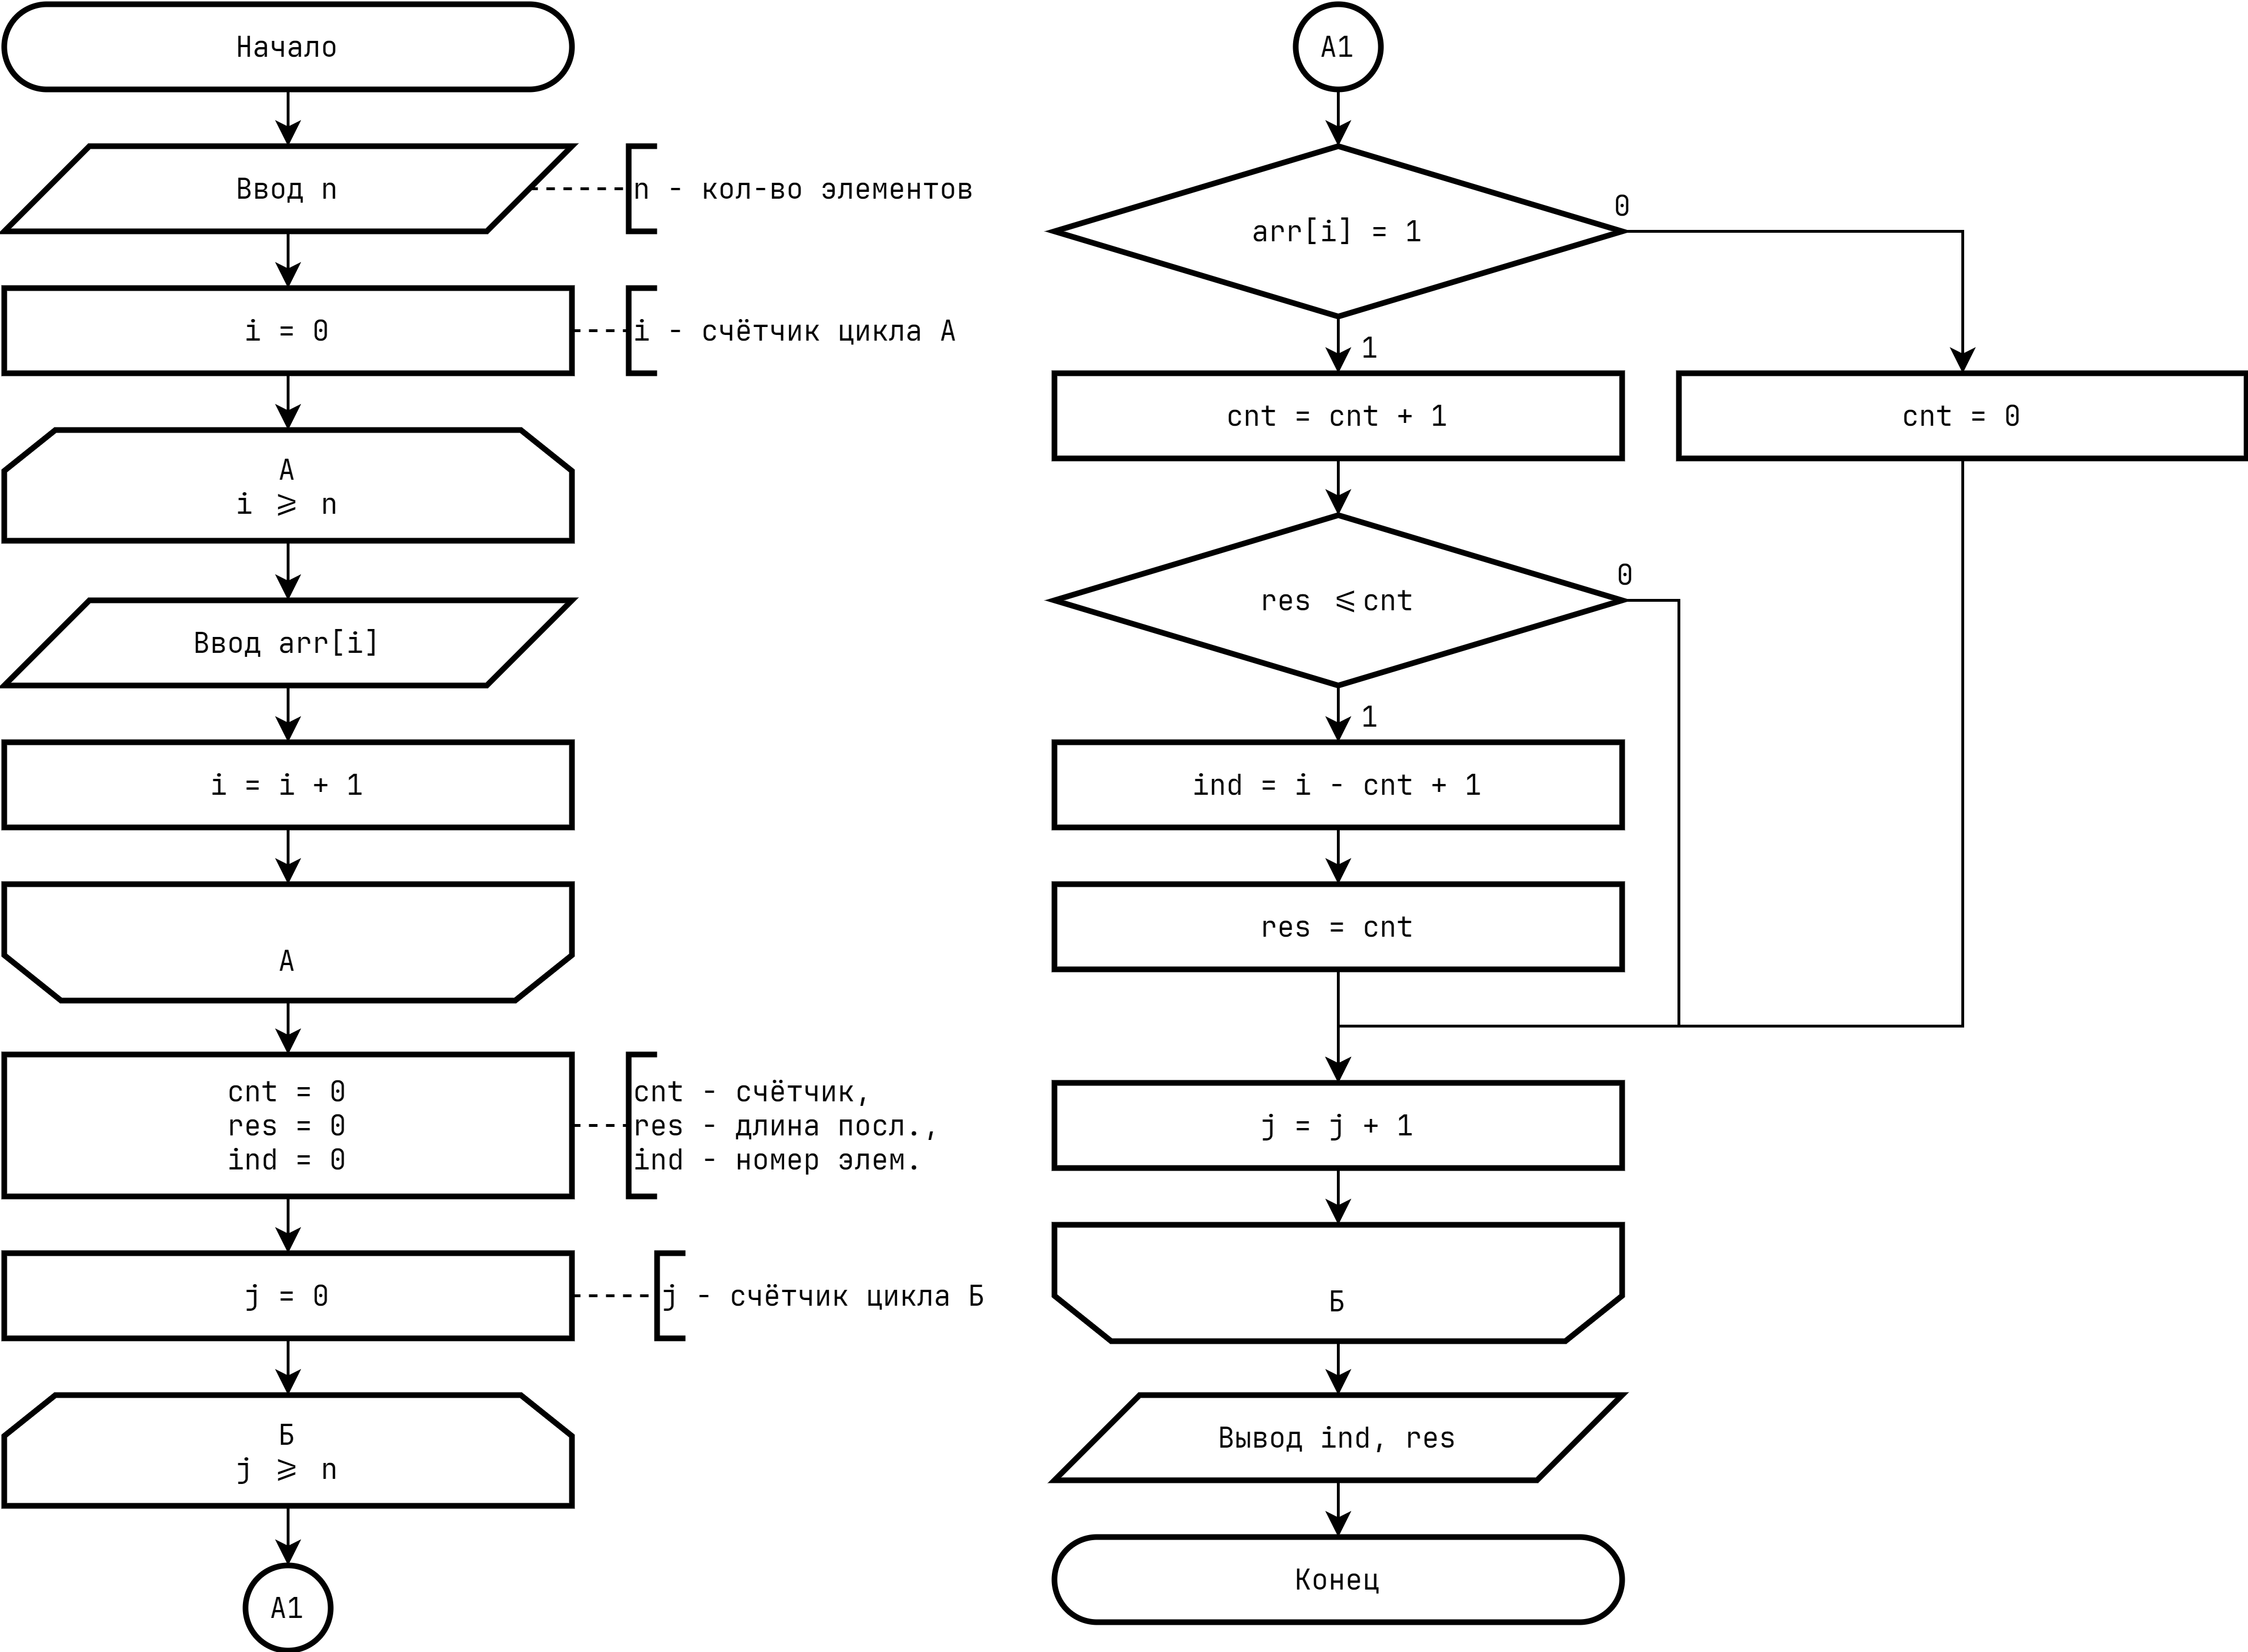
\includegraphics[width=0.8\textwidth]{pics/flowchart-15.png}
	\caption*{Рисунок 3 - Схема алгоритма Задания 3.}
\end{figure}

\section*{Задание 4.}
\noindent Схема алгоритма Задания 4 представлена на Рисунке 4.\\
\noindent Исходный код представлен в Приложении А4. \\
\newpage
\begin{figure}[!ht]
	\centering
	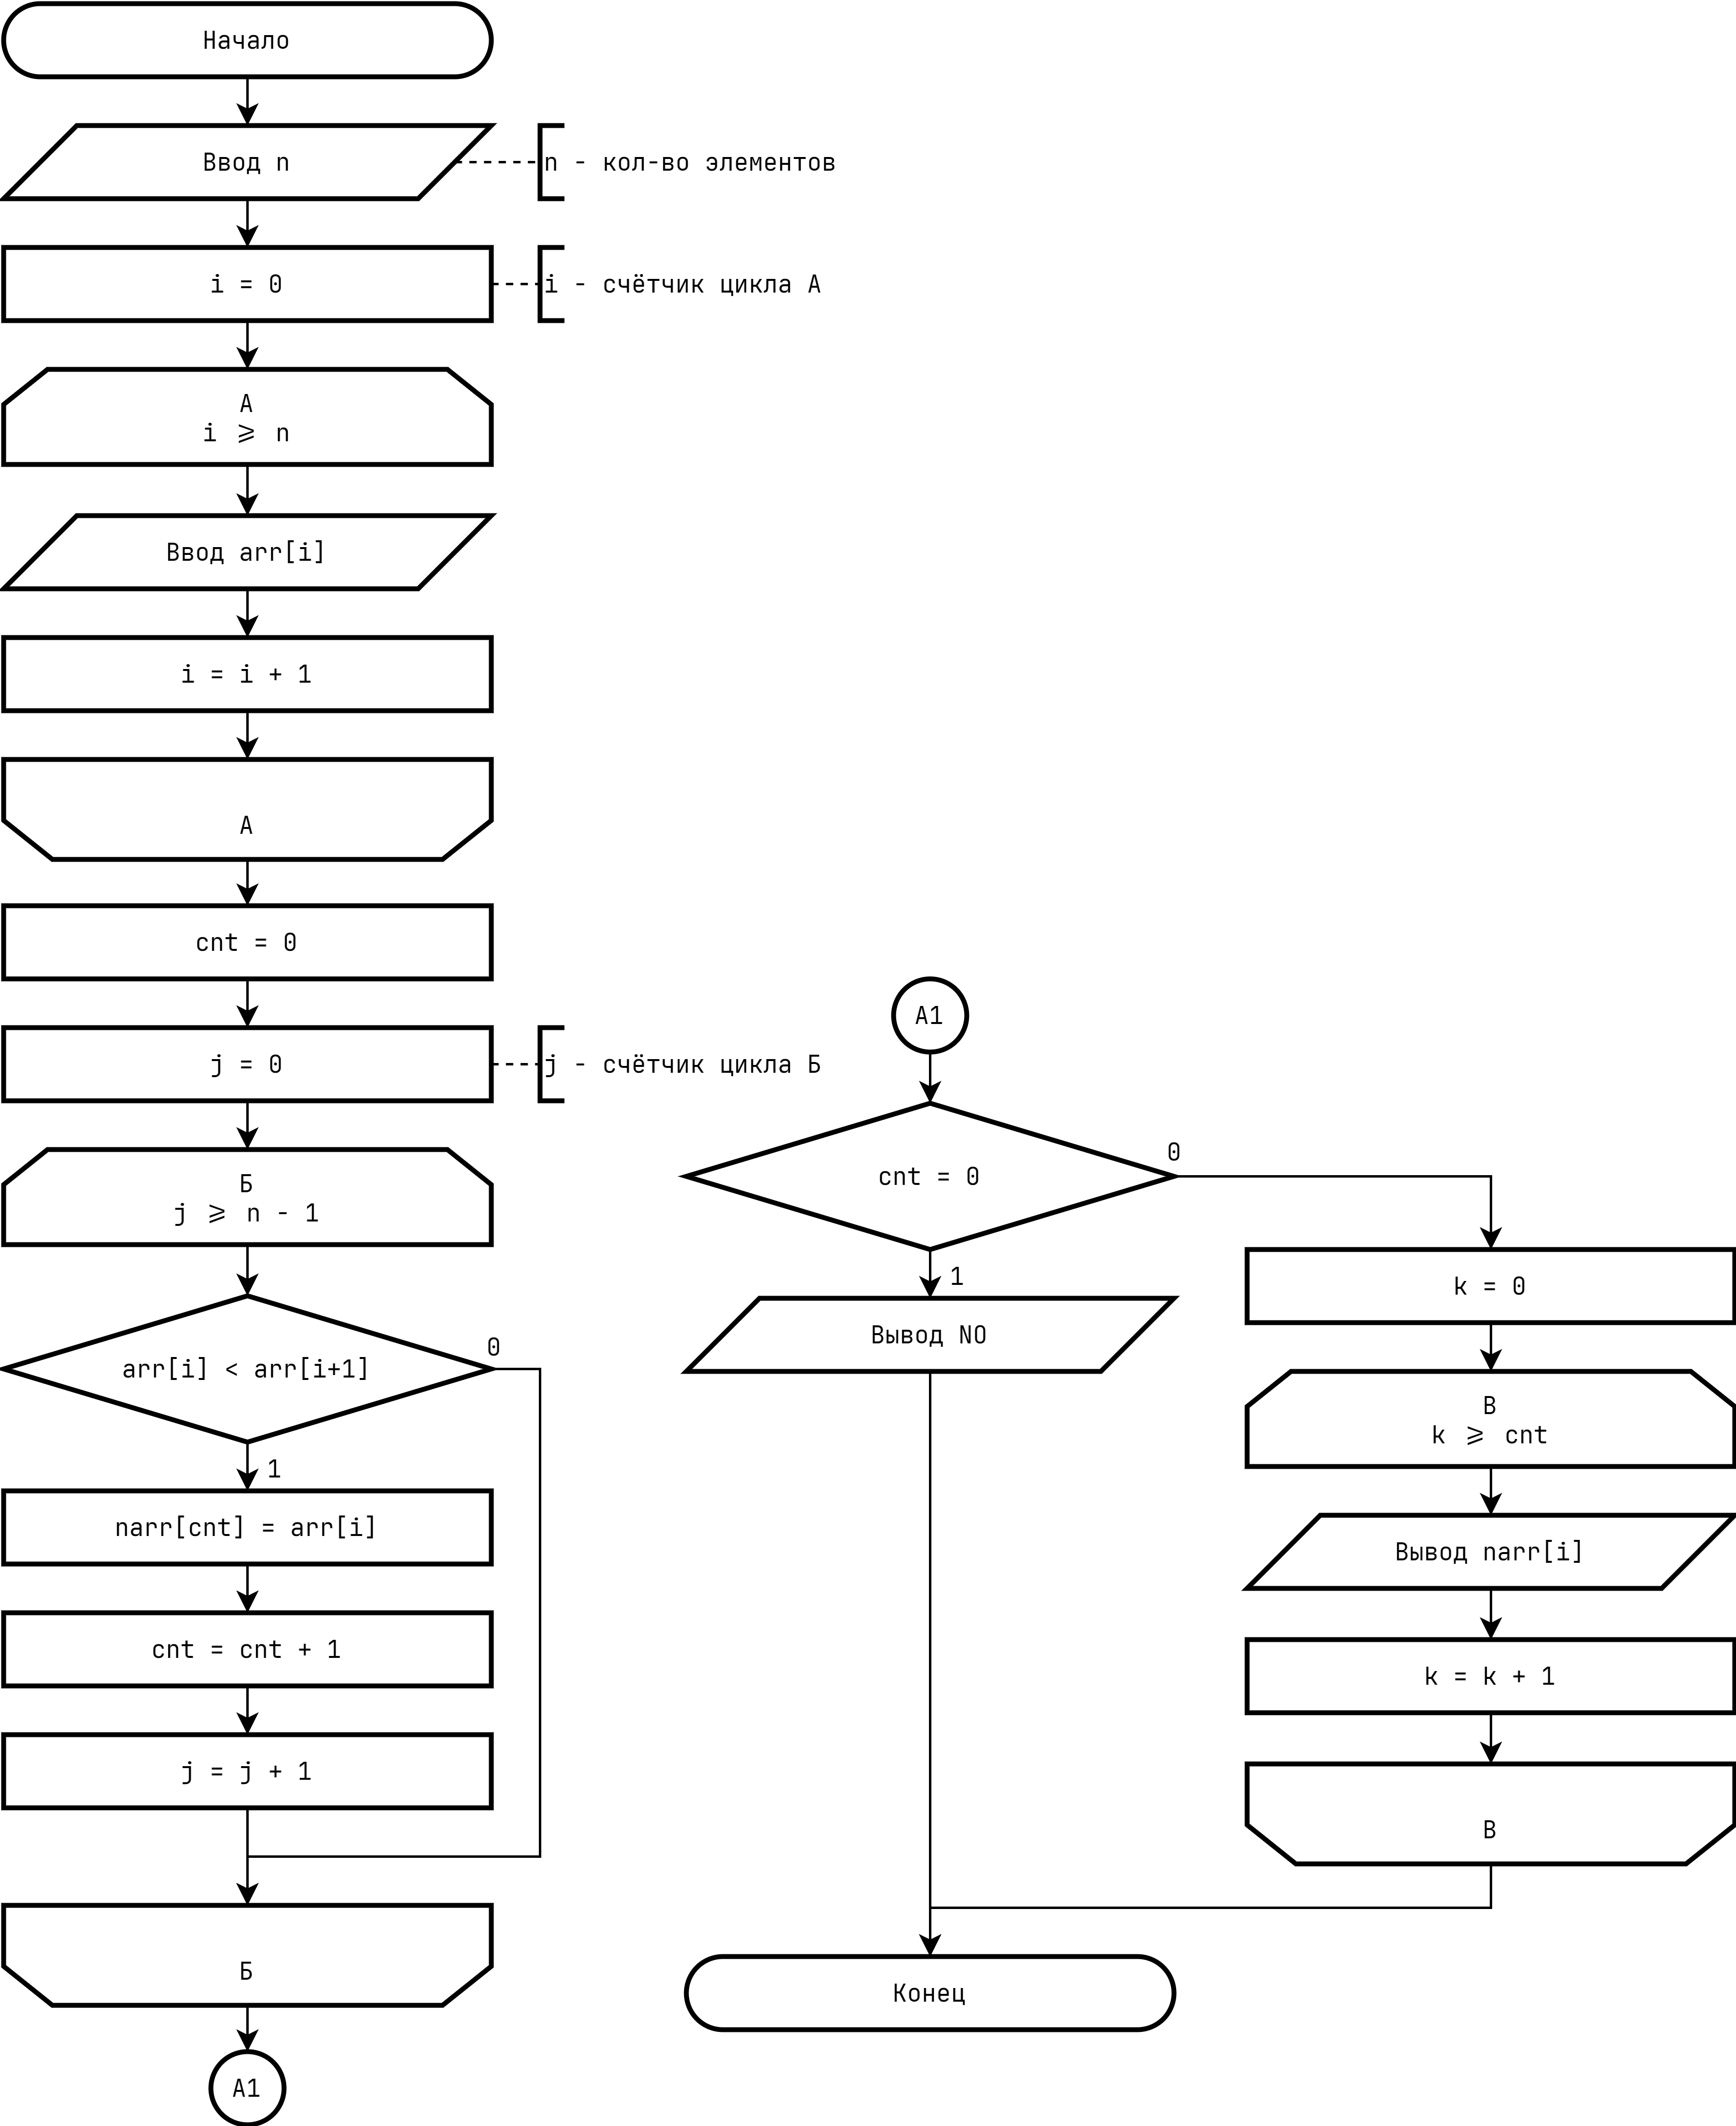
\includegraphics[width=0.75\textwidth]{pics/flowchart-16.png}
	\caption*{Рисунок 4 - Схема алгоритма Задания 4.}
\end{figure}

\section*{Задание 5.}
\noindent Схема алгоритма Задания 5 представлена на Рисунке 5.\\
\noindent Исходный код представлен в Приложении А5. \\

\begin{figure}[!ht]
	\centering
	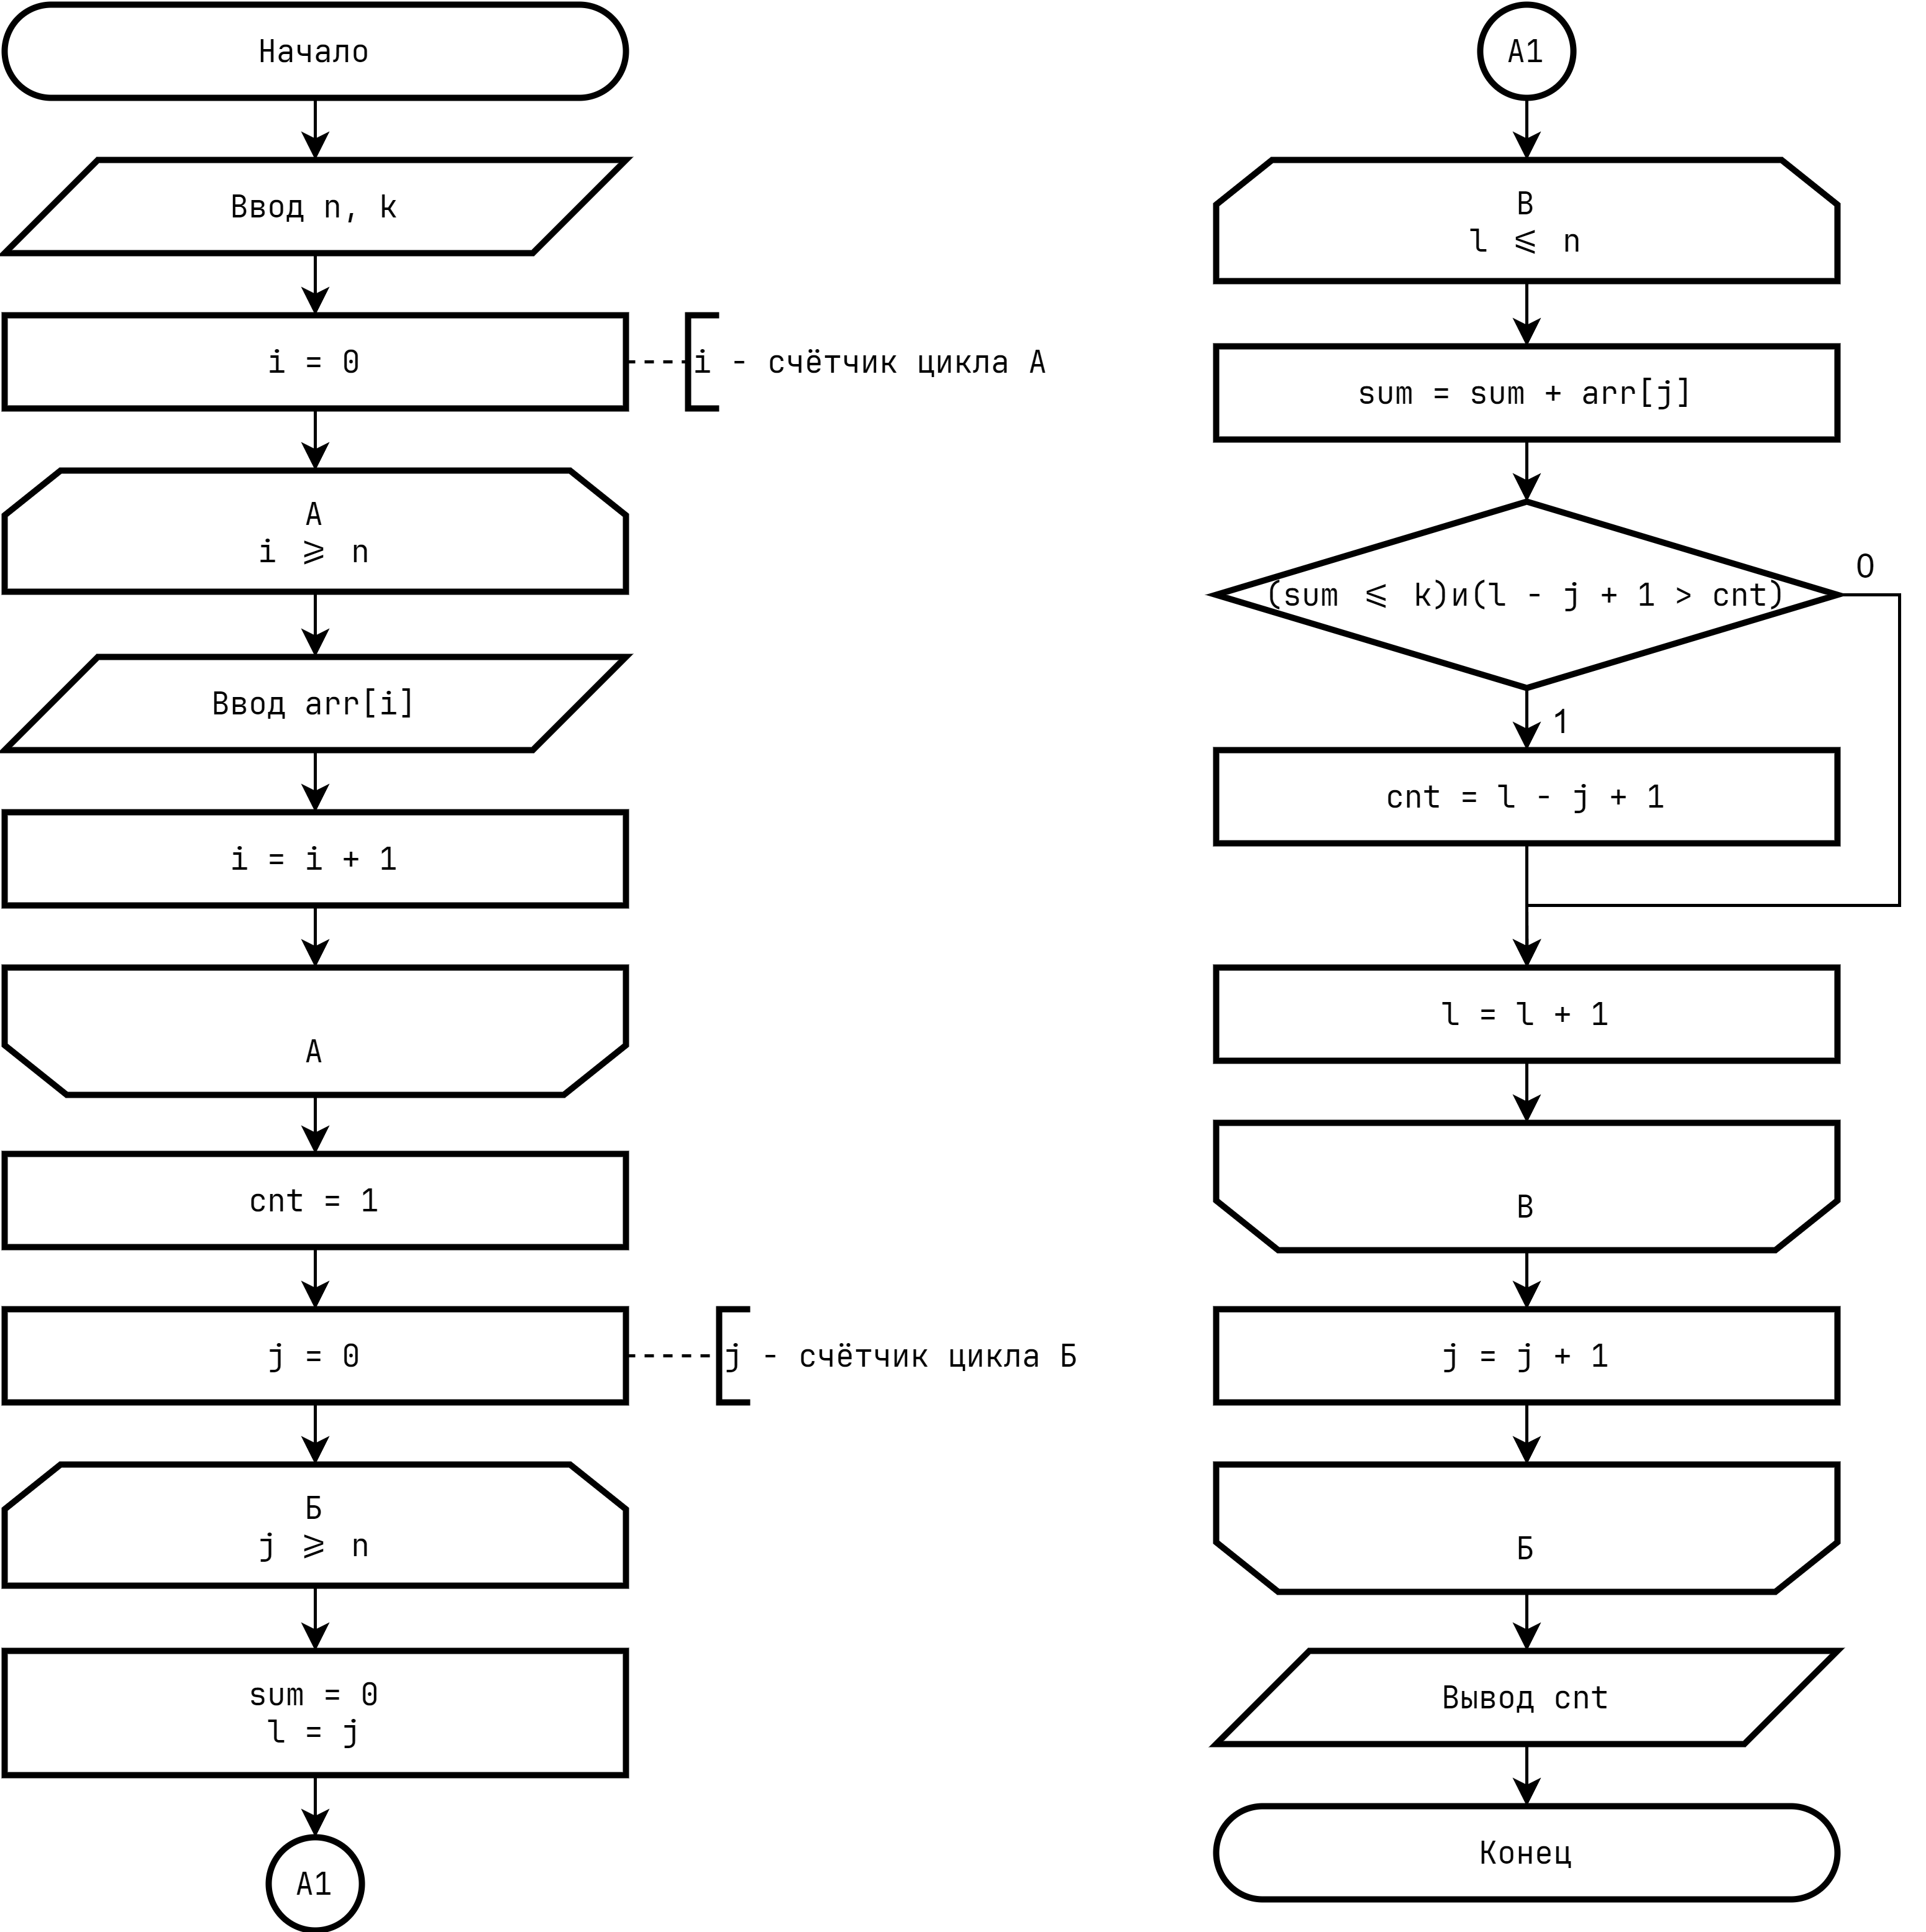
\includegraphics[width=0.75\textwidth]{pics/flowchart-17.png}
	\caption*{Рисунок 5 - Схема алгоритма Задания 5.}
\end{figure}

\section*{Задание 6.}
\noindent Схема алгоритма Задания 6 представлена на Рисунке 6.\\
\noindent Исходный код представлен в Приложении А6. \\
\newpage
\begin{figure}[!ht]
	\centering
	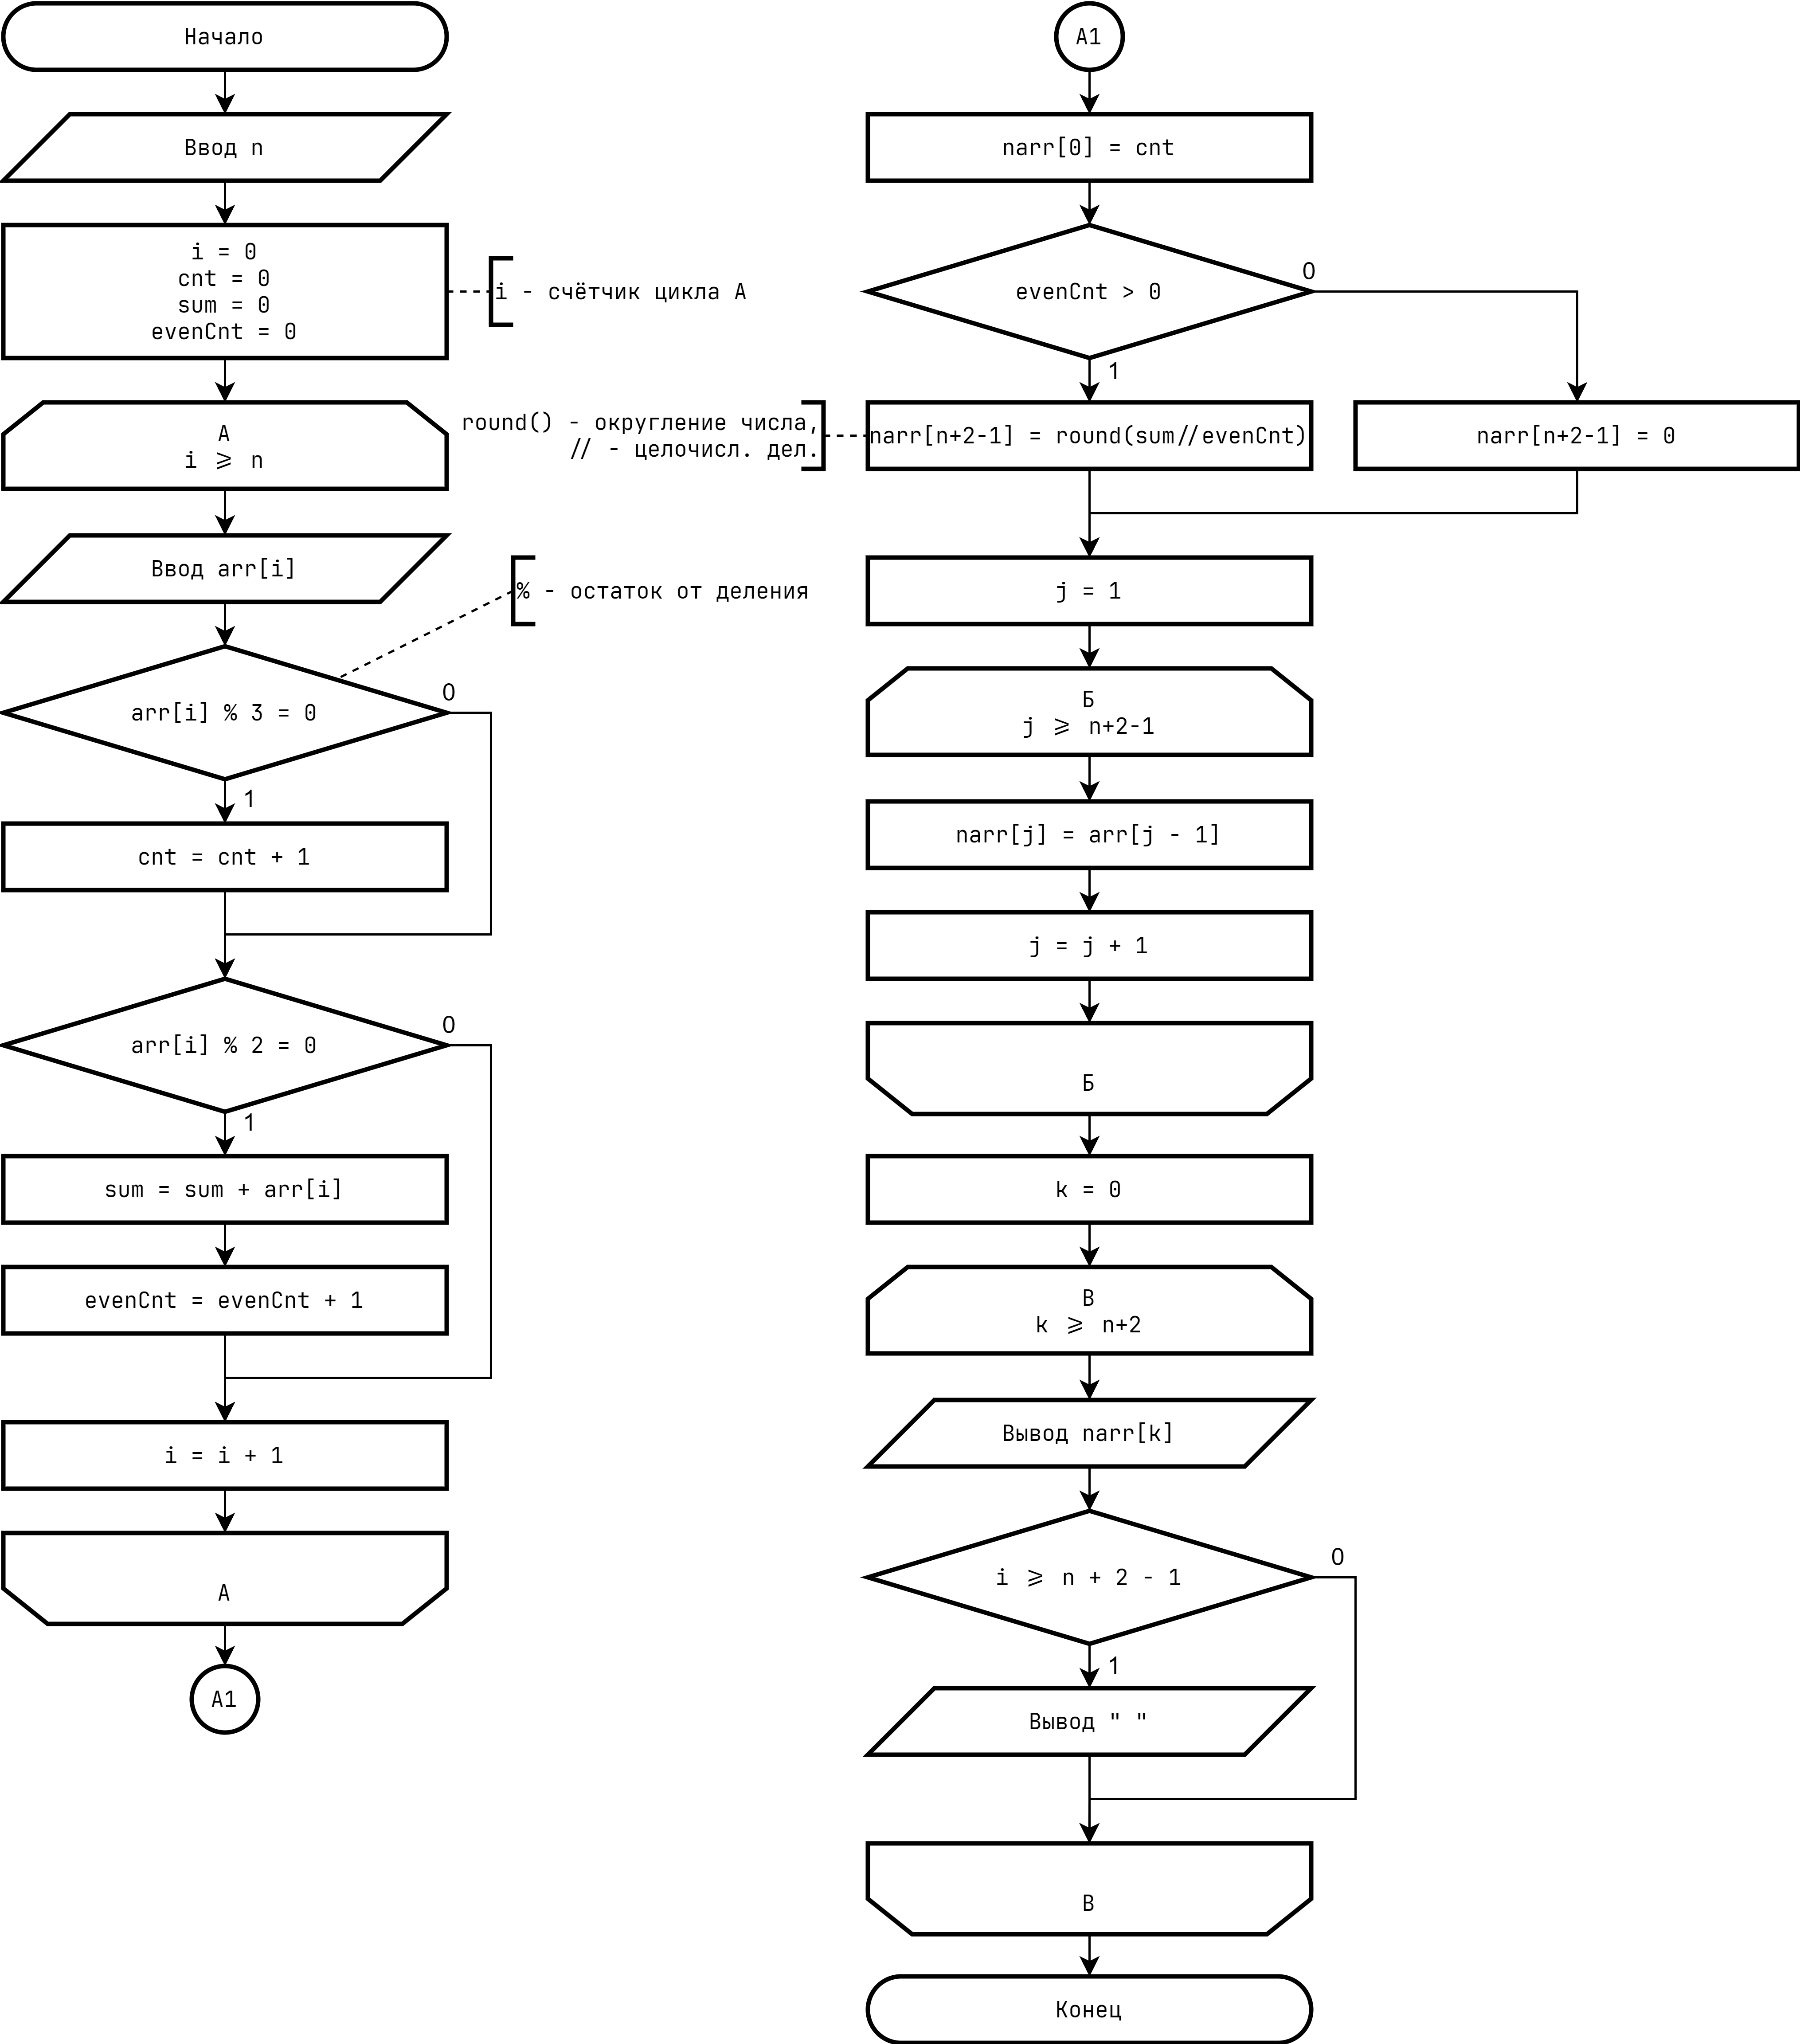
\includegraphics[width=0.8\textwidth]{pics/flowchart-18.png}
	\caption*{Рисунок 6 - Схема алгоритма Задания 6.}
\end{figure}

\section*{Задание 7.}
\noindent Схема алгоритма Задания 7 представлена на Рисунке 7.\\
\noindent Исходный код представлен в Приложении А7. \\
\newpage
\begin{figure}[!ht]
	\centering
	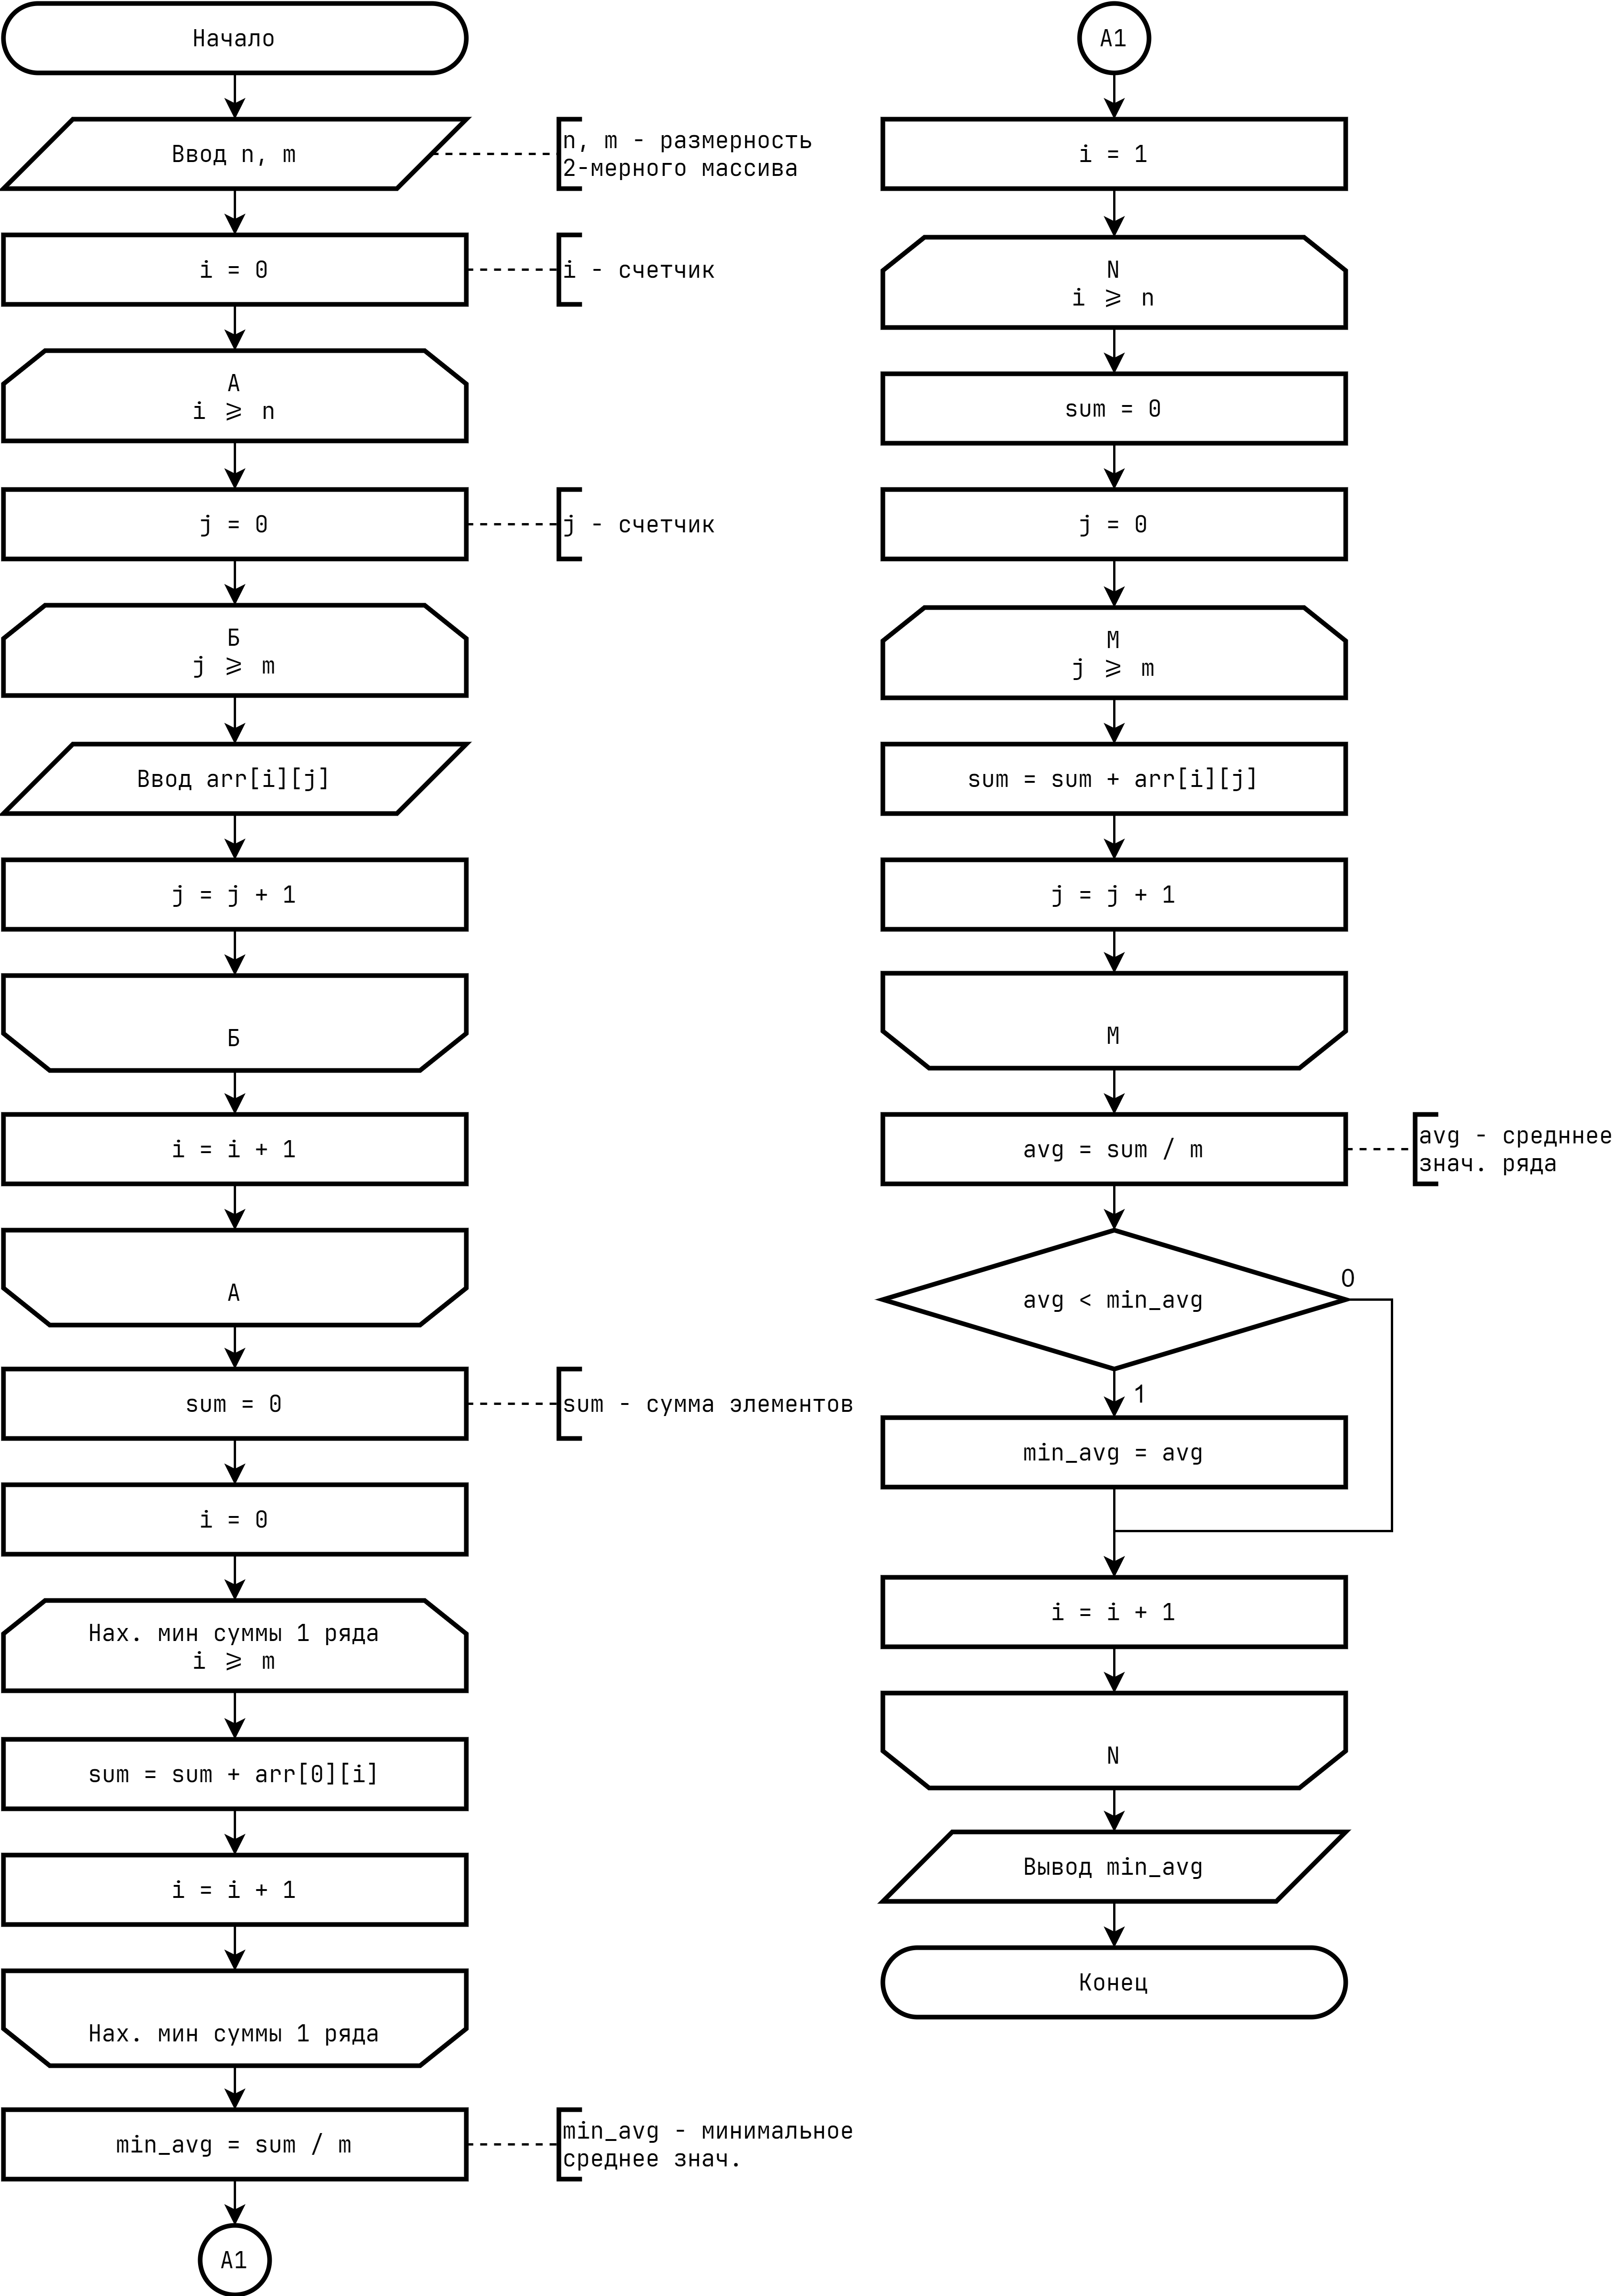
\includegraphics[width=0.75\textwidth]{pics/flowchart-19.png}
	\caption*{Рисунок 7 - Схема алгоритма Задания 7.}
\end{figure}

\section*{Задание 8.}
\noindent Схема алгоритма Задания 8 представлена на Рисунке 8.\\
\noindent Исходный код представлен в Приложении А8. \\
\begin{figure}[!ht]
	\centering
	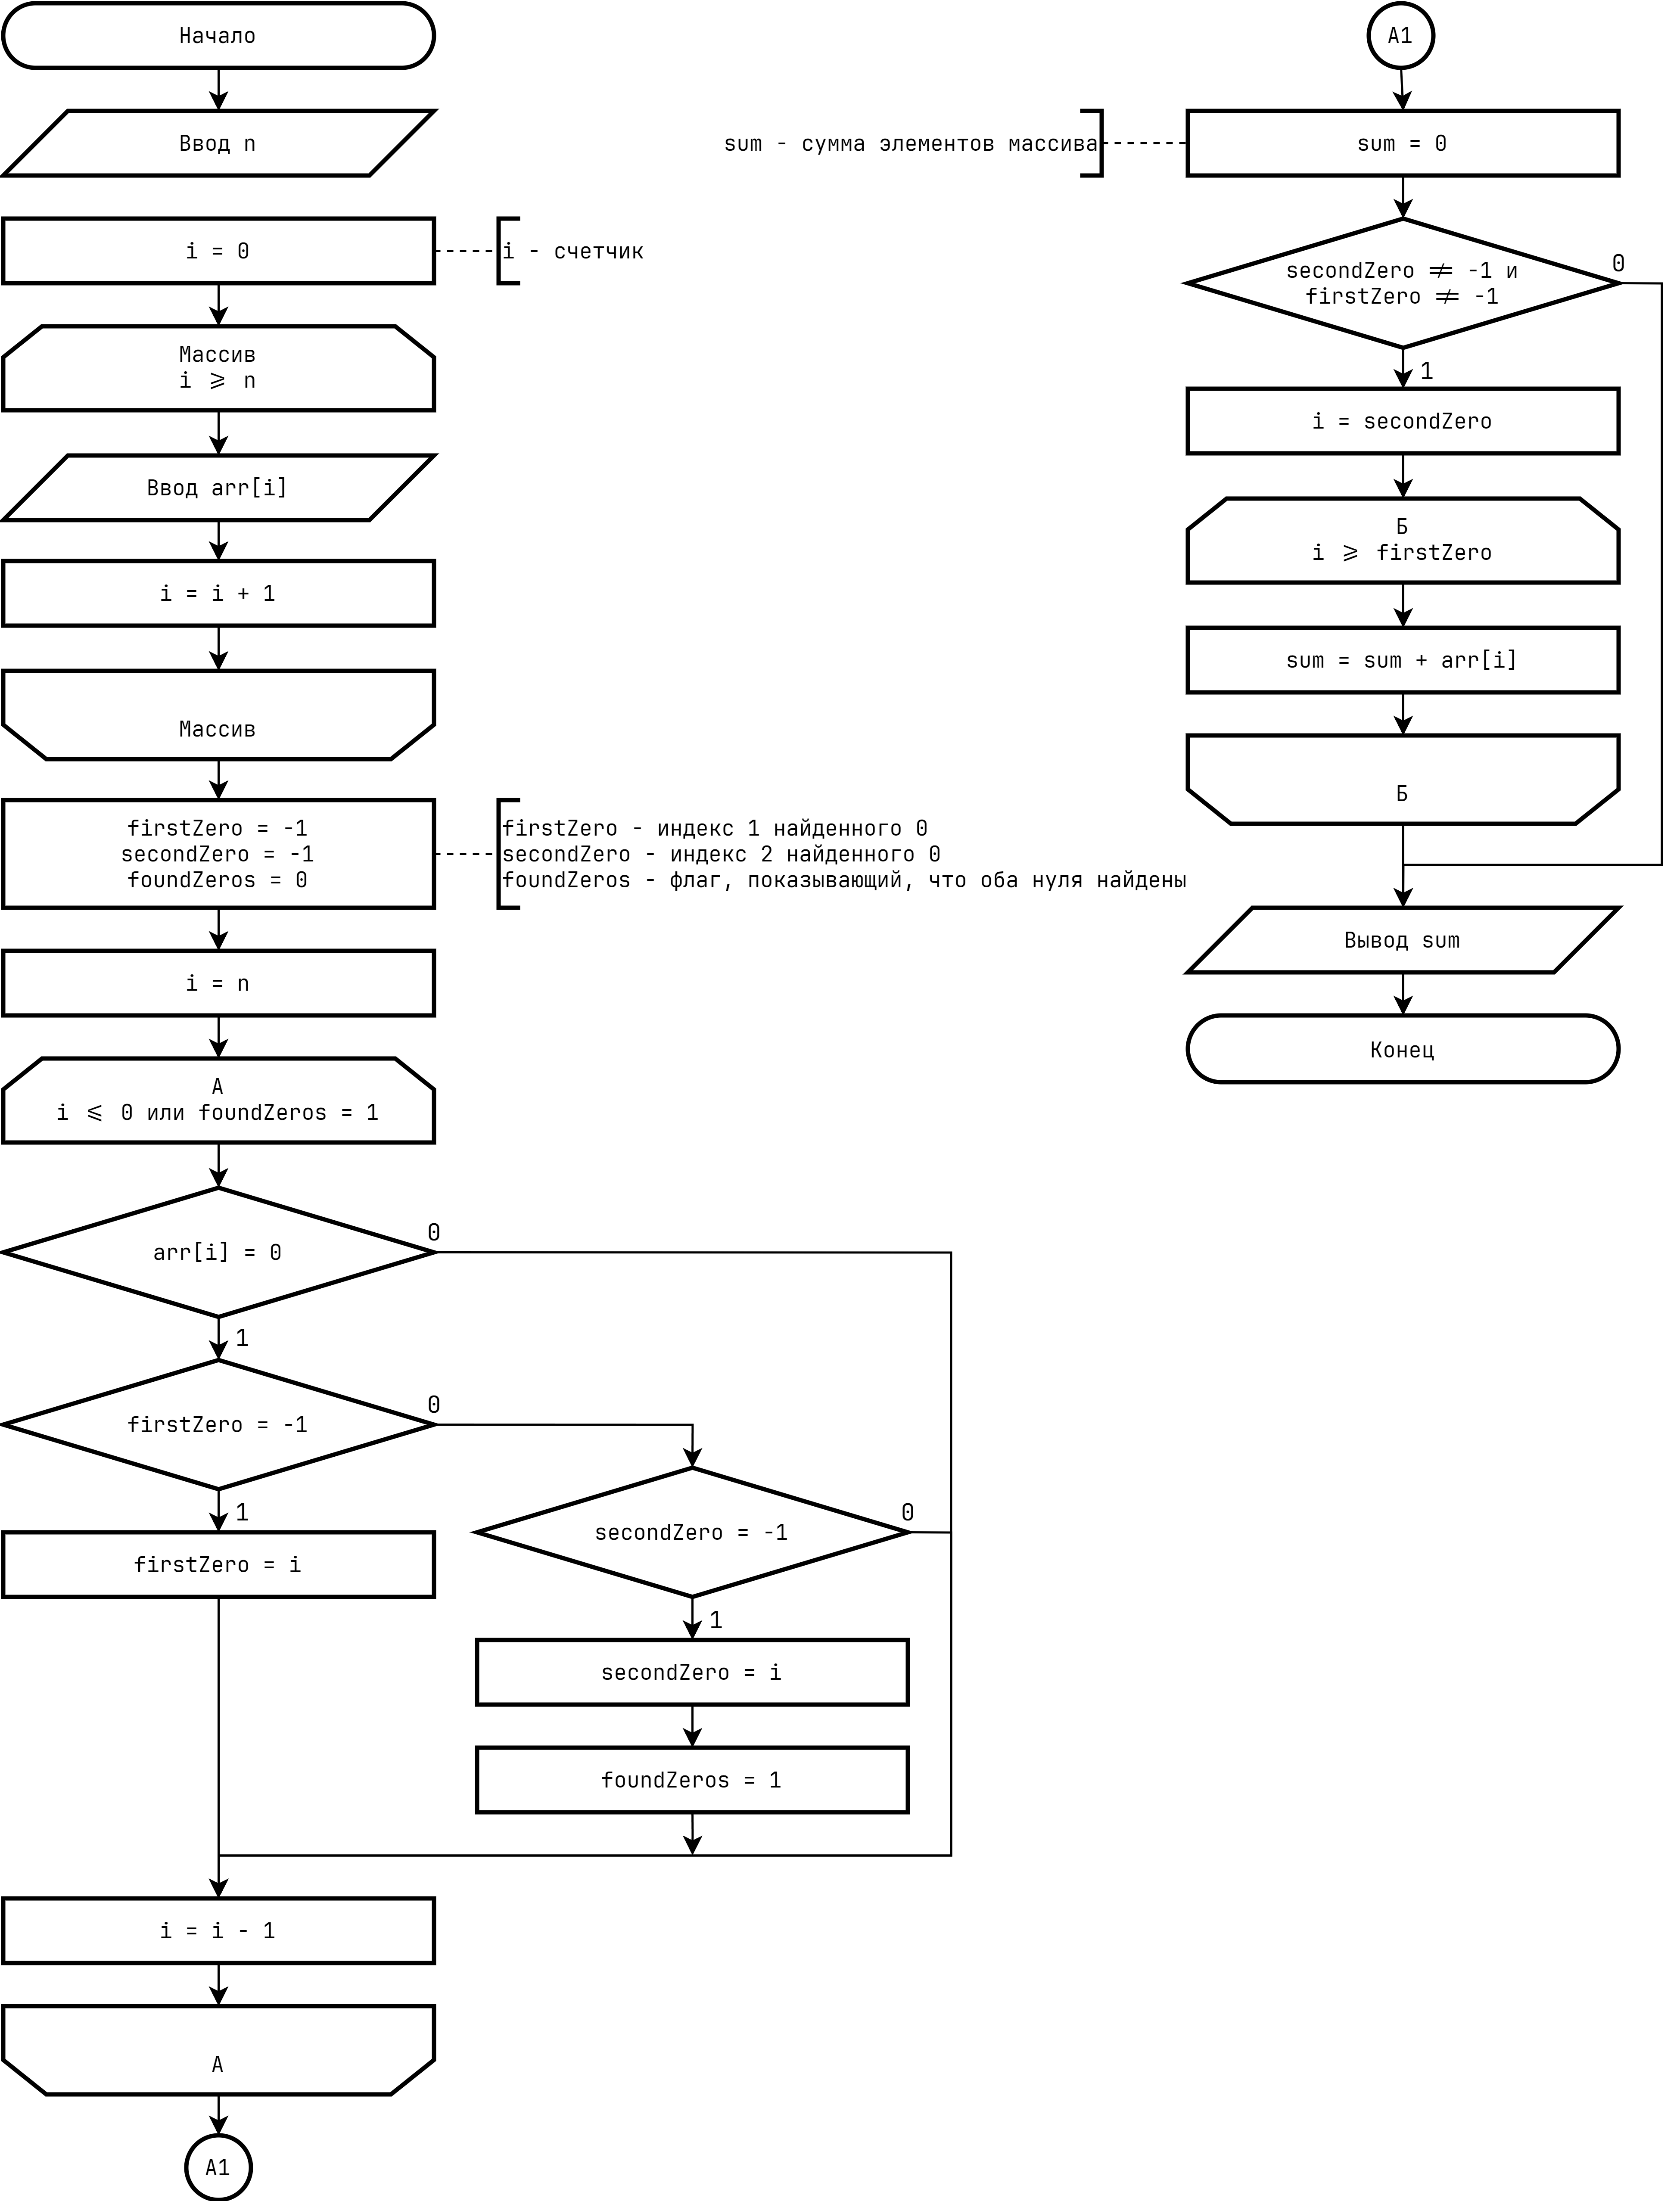
\includegraphics[width=0.75\textwidth]{pics/flowchart-20.png}
	\caption*{Рисунок 8 - Схема алгоритма Задания 8.}
\end{figure}

\section*{Задание 9.}
\noindent Схема алгоритма Задания 9 представлена на Рисунке 9.\\
\noindent Исходный код представлен в Приложении А9. \\
\begin{figure}[!ht]
	\centering
	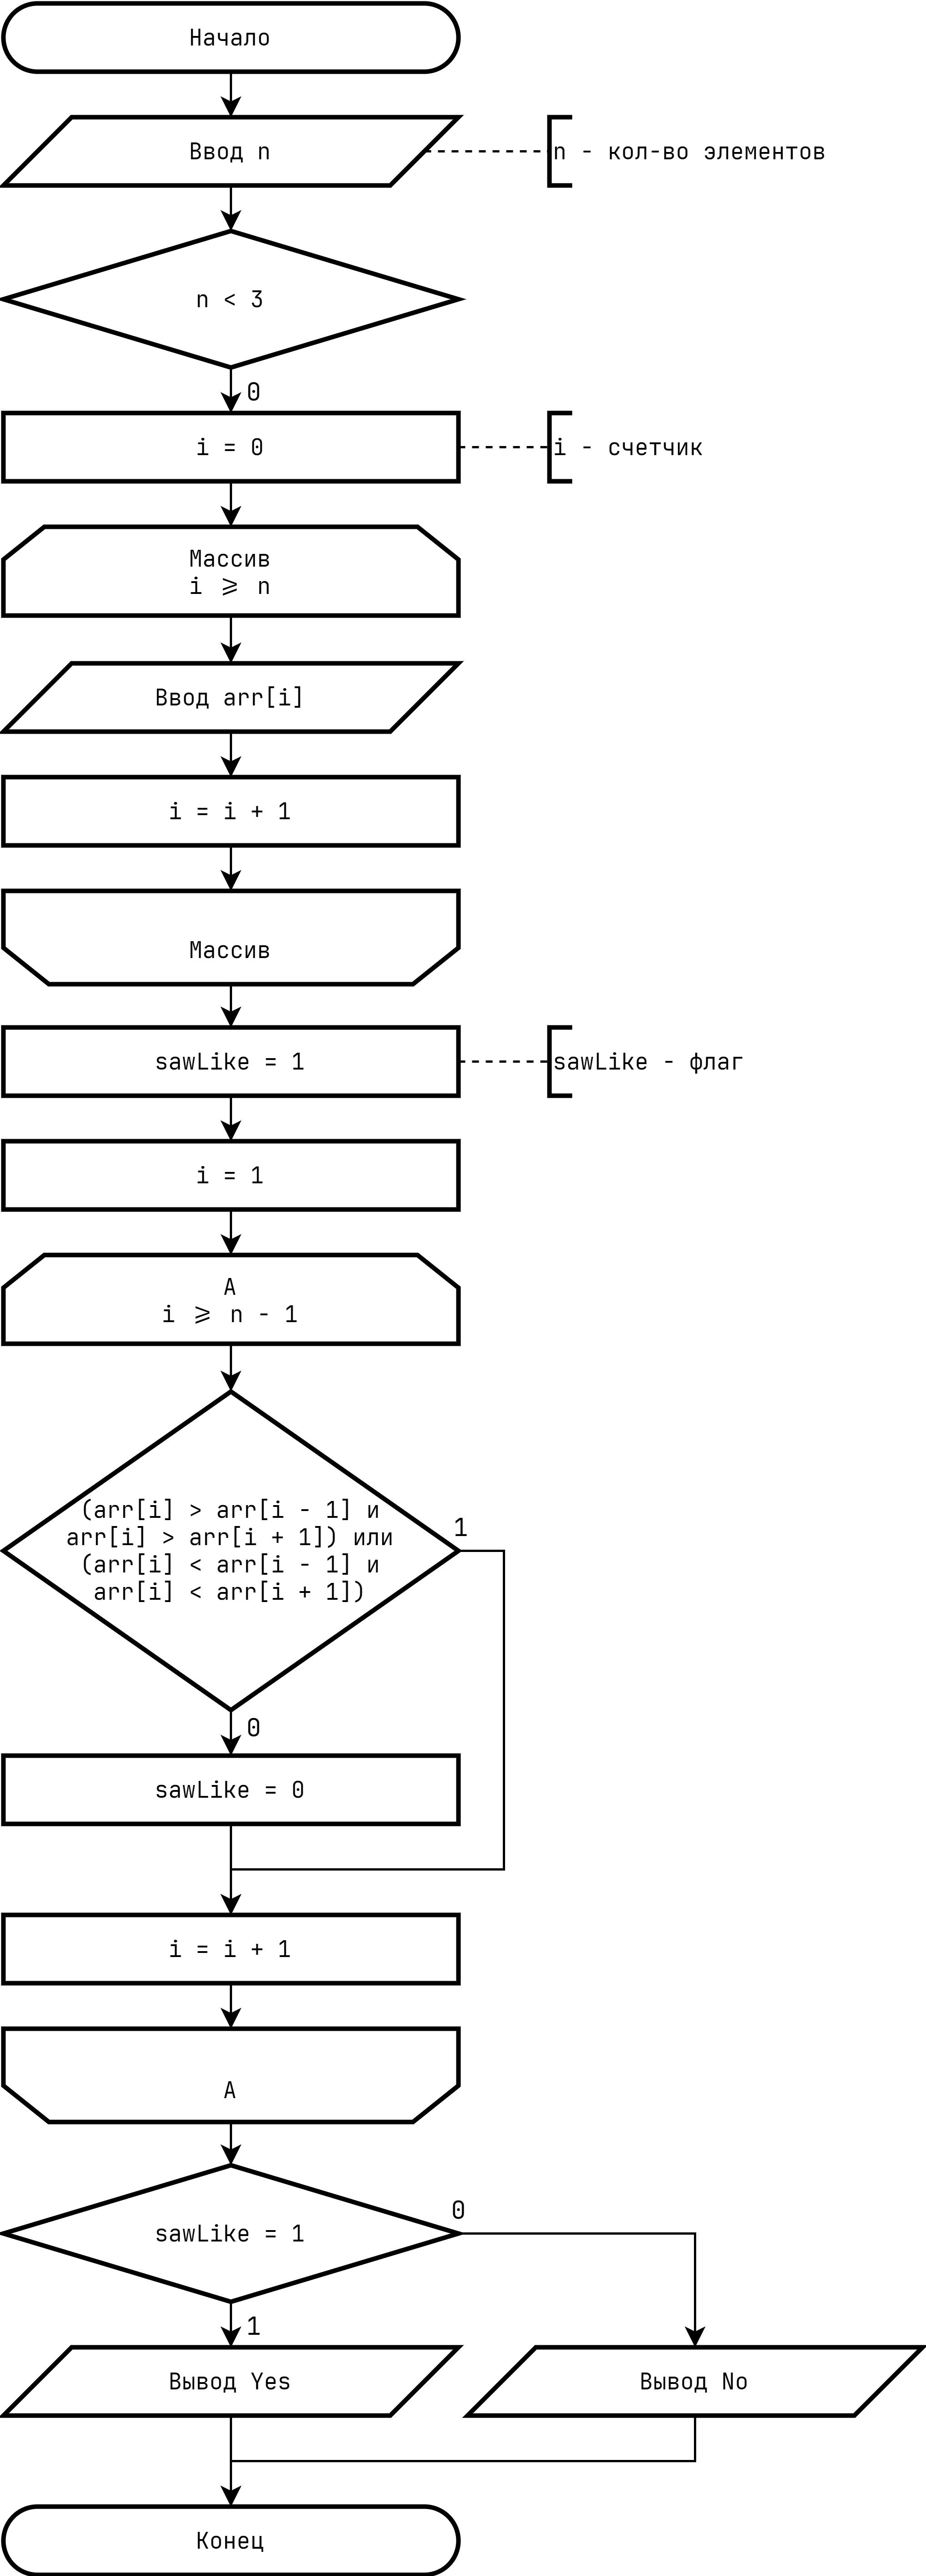
\includegraphics[height=0.75\textheight]{pics/flowchart-21.png}
	\caption*{Рисунок 9 - Схема алгоритма Задания 9.}
\end{figure}

\section*{Задание 10.}
\noindent Схема алгоритма Задания 10 представлена на Рисунке 10.\\
\noindent Исходный код представлен в Приложении А10. \\
\begin{figure}[!ht]
	\centering
	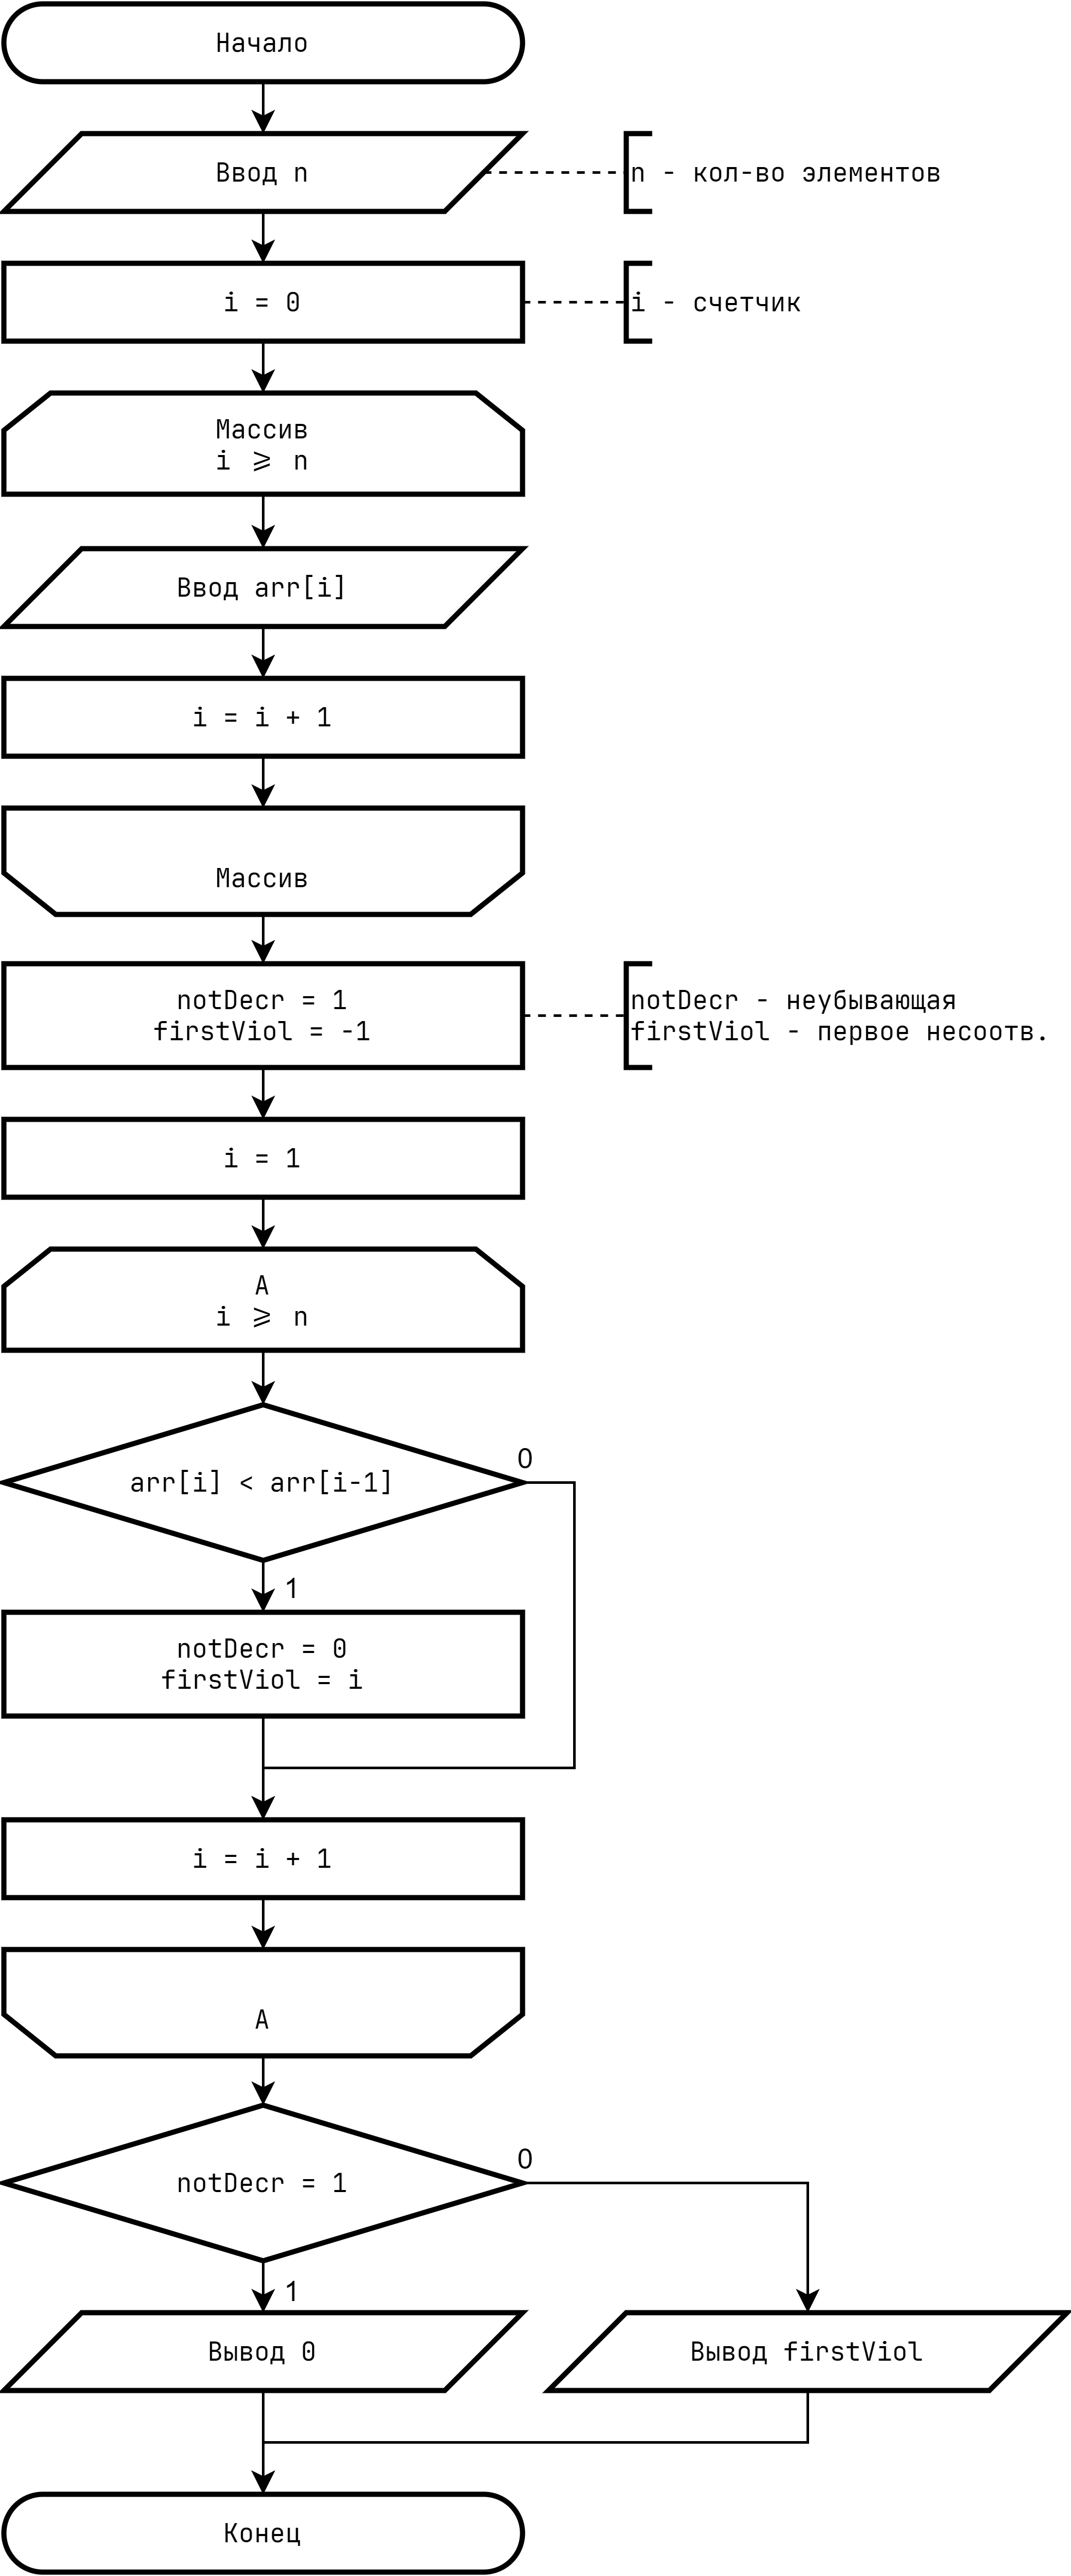
\includegraphics[height=0.75\textheight]{pics/flowchart-22.png}
	\caption*{Рисунок 10 - Схема алгоритма Задания 10.}
\end{figure}


\section*{Приложеие А1. Исходный код для Задания 1.}
\VerbatimInput[fontsize=\small]{code/C/13.c}
\section*{Приложение А2. Исходный код для Задания 2.}
\VerbatimInput[fontsize=\small]{code/pas/14.pas}
\section*{Приложение А3. Исходный код для Задания 3.}
\VerbatimInput[fontsize=\small]{code/C/15.c}
\section*{Приложение А4. Исходный код для Задания 4.}
\VerbatimInput[fontsize=\small]{code/pas/16.pas}
\section*{Приложение А5. Исходный код для Задания 5.}
\VerbatimInput[fontsize=\small]{code/C/17.c}
\section*{Приложение А6. Исходный код для Задания 6.}
\VerbatimInput[fontsize=\small]{code/pas/18.pas}
\section*{Приложение А7. Исходный код для Задания 7.}
\VerbatimInput[fontsize=\small]{code/C/19.c}
\section*{Приложение А8. Исходный код для Задания 8.}
\VerbatimInput[fontsize=\small]{code/pas/20.pas}
\section*{Приложение А9. Исходный код для Задания 9.}
\VerbatimInput[fontsize=\small]{code/C/21.c}
\section*{Приложение А10. Исходный код для Задания 10.}
\VerbatimInput[fontsize=\small]{code/pas/22.pas}

\section*{Вывод}
В ходе выполнения лабораторной работы были изучены и реализованы алгоритмы
обработки одномерных массивов и матриц на языках программирования Pascal и C.
Работа включала решения задач различного уровня сложности, направленных на
развитие навыков алгоритмического мышления, обработки данных и анализа
результатов.\\

\end{document}